\documentclass[french,11pt]{beamer}

\DeclareMathOperator{\Cov}{Cov}
\DeclareMathOperator{\Var}{Var}
\DeclareMathOperator{\E}{\mathbb{E}}
\DeclareMathOperator{\Proba}{\mathbb{P}}

\newcommand{\Covb}[2]{\ensuremath{\Cov\!\left[#1,#2\right]}}
\newcommand{\Eb}[1]{\ensuremath{\E\!\left[#1\right]}}
\newcommand{\Pb}[1]{\ensuremath{\Proba\!\left[#1\right]}}
\newcommand{\Varb}[1]{\ensuremath{\Var\!\left[#1\right]}}

% norm
\newcommand{\norm}[1]{\| #1 \|}

\newcommand{\indep}{\rotatebox[origin=c]{90}{$\models$}}





\usepackage{mathptmx,amsmath,amssymb,graphicx,bibentry,bbm,babel,ragged2e}

\makeatletter

\newcommand{\noun}[1]{\textsc{#1}}
\newcommand{\jitem}[1]{\item \begin{justify} #1 \end{justify} \vfill{}}
\newcommand{\sframe}[2]{\frame{\frametitle{#1} #2}}

\newenvironment{centercolumns}{\begin{columns}[c]}{\end{columns}}
%\newenvironment{jitem}{\begin{justify}\begin{itemize}}{\end{itemize}\end{justify}}

\usetheme{Warsaw}
\setbeamertemplate{footline}[text line]{}
\setbeamercolor{structure}{fg=purple!50!blue, bg=purple!50!blue}

\setbeamersize{text margin left=15pt,text margin right=15pt}

\setbeamercovered{transparent}


\@ifundefined{showcaptionsetup}{}{%
 \PassOptionsToPackage{caption=false}{subfig}}
\usepackage{subfig}

\usepackage[utf8]{inputenc}
\usepackage[T1]{fontenc}



\makeatother

\begin{document}


\title{Génération de Données Synthétiques Corrélées}

\author{J.~Raimbault$^{1,2}$\\
\texttt{juste.raimbault@parisgeo.cnrs.fr}
}


\institute{$^{1}$UMR CNRS 8504 G{\'e}ographie-cit{\'e}s\\
$^{2}$UMR-T IFSTTAR 9403 LVMT\\
}


\date{Journées de Rochebrune 2016\\\smallskip
\textit{Nature des données, théorie de la donnée I : perspective méthodologique}\\\smallskip
Mercredi 20 janvier 2016
}

\frame{\maketitle}


%%%%%%%%%%%%%%%%%
\section{Introduction}
%%%%%%%%%%%%%%%%%


%%%%%%%%%%%%%%%%%
\subsection{Introduction}
%%%%%%%%%%%%%%%%%


%%%%%%%%%%%%%%%%%
\sframe{Un problème fondamental...}{
\textbf{Experience de pensée : }

Les relations skieurs/snowboardeurs sont devenues ces derniers jours un réel problème de société. La station dispose d'une marge de manoeuvre très faible, par exemple :
\begin{itemize}
\item politique de zonage (spatial ou temporel) pour limiter les interactions
\item campagnes de sensibilisations pour jouer sur paramètres individuels
\end{itemize}

\medskip

\textit{Comment évaluer ces mesures de manière prospective ? }

\textbf{$\mathbf{\rightarrow}$ Modéliser !}

\bigskip

(exemple incongru : utilisateurs de VLib dans~\cite{raimbault2015user} ! )
}
%%%%%%%%%%%%%%%%%%%%%%%%%%%%


%%%%%%%%%%%%%%%%%
\sframe{... à la solution simple...}{
\textbf{(Suite de l'expérience)}

\medskip

On suppose avoir construit (avec ou sans UML) et implémenté un modèle de simulation stochastique (agent ou non), qui étant donné l'organisation spatiale d'une station et une population pratiquant les sports d'hiver (paramètres laissés à votre imagination), simule le déroulement d'une journée de ski et produit des indicateurs de performance/statisfaction.

\bigskip

$\rightarrow$\textit{L'intégration des actions possibles de la station dans le modèle permettrait d'évaluer leur impact sur l'amélioration des conflits ski/snow ?}


}


%%%%%%%%%%%%%%%%%
\sframe{mais finalement complexe ?}{

\begin{itemize}
\jitem{L'exploration intensive des modèles de simulation (comportement statistique, analyse de sensibilité, exploration de l'espace des paramètres, calibration, etc.) est essentielle pour en tirer de la connaissance\\\cite{rey2015plateforme,banos2013pour}}
\jitem{Cela inclut la sensibilité \emph{aux conditions initiales}, ex. : topographie et configuration de la station, composition de la population ; au premier ordre (distribution des données en elle-mêmes) mais aussi \emph{au second ordre} (covariation des données ; ex. : correlation entre les capacités des snowboarders à prendre un téléski et la haine des skieurs).}
\end{itemize}

$\rightarrow$ d'où la nécessité de générer des \emph{jeux de données} artificiels, ou \emph{données synthétiques}, contrôlées au différents ordres, pour une exploration complète du modèle.

}




%%%%%%%%%%%%%%%%%
\subsection{Problématique}
%%%%%%%%%%%%%%%%%

\sframe{Contexte}{
\textbf{Def. : } Des \emph{données synthétiques} sont dans notre cas des sorties de modèles génératifs (et possiblement des entrées des modèles qui les utilisent).
\medskip

Méthodologie utilisée dans de nombreux domaines, par ex. évaluation thérapeutique~\cite{abadie2010synthetic}, étude des systèmes territoriaux~\cite{moeckel2003creating,pritchard2009advances}, apprentissage statistique~\cite{bolon2013review} ou la bio-informatique~\cite{van2006syntren}.

\medskip

Peu répandu au second ordre : exemples spécifiques comme~\cite{ye2011investigation} pour choix discrets ; méthodes pouvant être interprétées comme telles : generation de réseaux complexes~\cite{newman2003structure}.

}




%%%%%%%%%%%%%%%%%
\section{Méthode}
%%%%%%%%%%%%%%%%%


%%%%%%%%%%%%%%%%%
\sframe{Méthode générique proposée}{
$\vec{X}_I$ processus stochastique multidimensionnel, $\mathbf{X}=(X_{i,j})$ jeu de réalisations. 

\bigskip

\textbf{But : } Générer une population statistique $\mathbf{\tilde{X}}=\tilde{X}_{i,j}$ telle que :
\medskip
\begin{enumerate}
\item critère de proximité aux données : étant donné une précision $\varepsilon$ et un indicateur $f$, $\norm{f(\mathbf{X})-f(\mathbf{\tilde{X}})} < \varepsilon$
\item contrôle de la structure de correlation estimée : $\hat{\Var{}}\left[(\tilde{X}_i)\right] = \Sigma R$ avec $R$ fixé.
\end{enumerate}

}



%%%%%%%%%%%%%%%%%
\section{Applications}
%%%%%%%%%%%%%%%%%

%%%%%%%%%%%%%%%%%
\subsection{Séries Temporelles Financières}
%%%%%%%%%%%%%%%%%


%%%%%%%%%%%%%%%%%
\sframe{Application : Finance Quantitative}{

\begin{itemize}
\jitem{Séries temporelles financières, signaux typiques de systèmes complexes hétérogènes et multiscalaires~\cite{mantegna2000introduction}.}
\jitem{Etude des correlations entre actifs centrale à de nombreuses approches : Matrices aléatoires~\cite{2009arXiv0910.1205B}, réseaux complexes \cite{2001PhyA..299...16B} \cite{tumminello2005tool}, dérivations théorique d'estimateurs spécifiques~\cite{barndorff2011multivariate}}
\jitem{Données synthétiques corrélées utilisées dans cas simples 
\cite{potiron2015estimation} : validation de résultats théoriques, performance d'un modèle prédictif.}
\end{itemize}






}



%%%%%%%%%%%%%%%%%
\sframe{Formalisation}{
Réseau d'actif $(X_i(t))_{1\leq i \leq N}$ interprétés comme signaux multiscalaires : $X_i=\sum_{\omega}{X_i^{\omega}}$. On notera $T_i^{\omega} = \sum_{\omega' \leq \omega} X_i^{\omega}$.

\medskip

Dynamique de Black-Scholes $dX = \sigma\cdot dW$ avec $W$ processus de Wiener

\centering
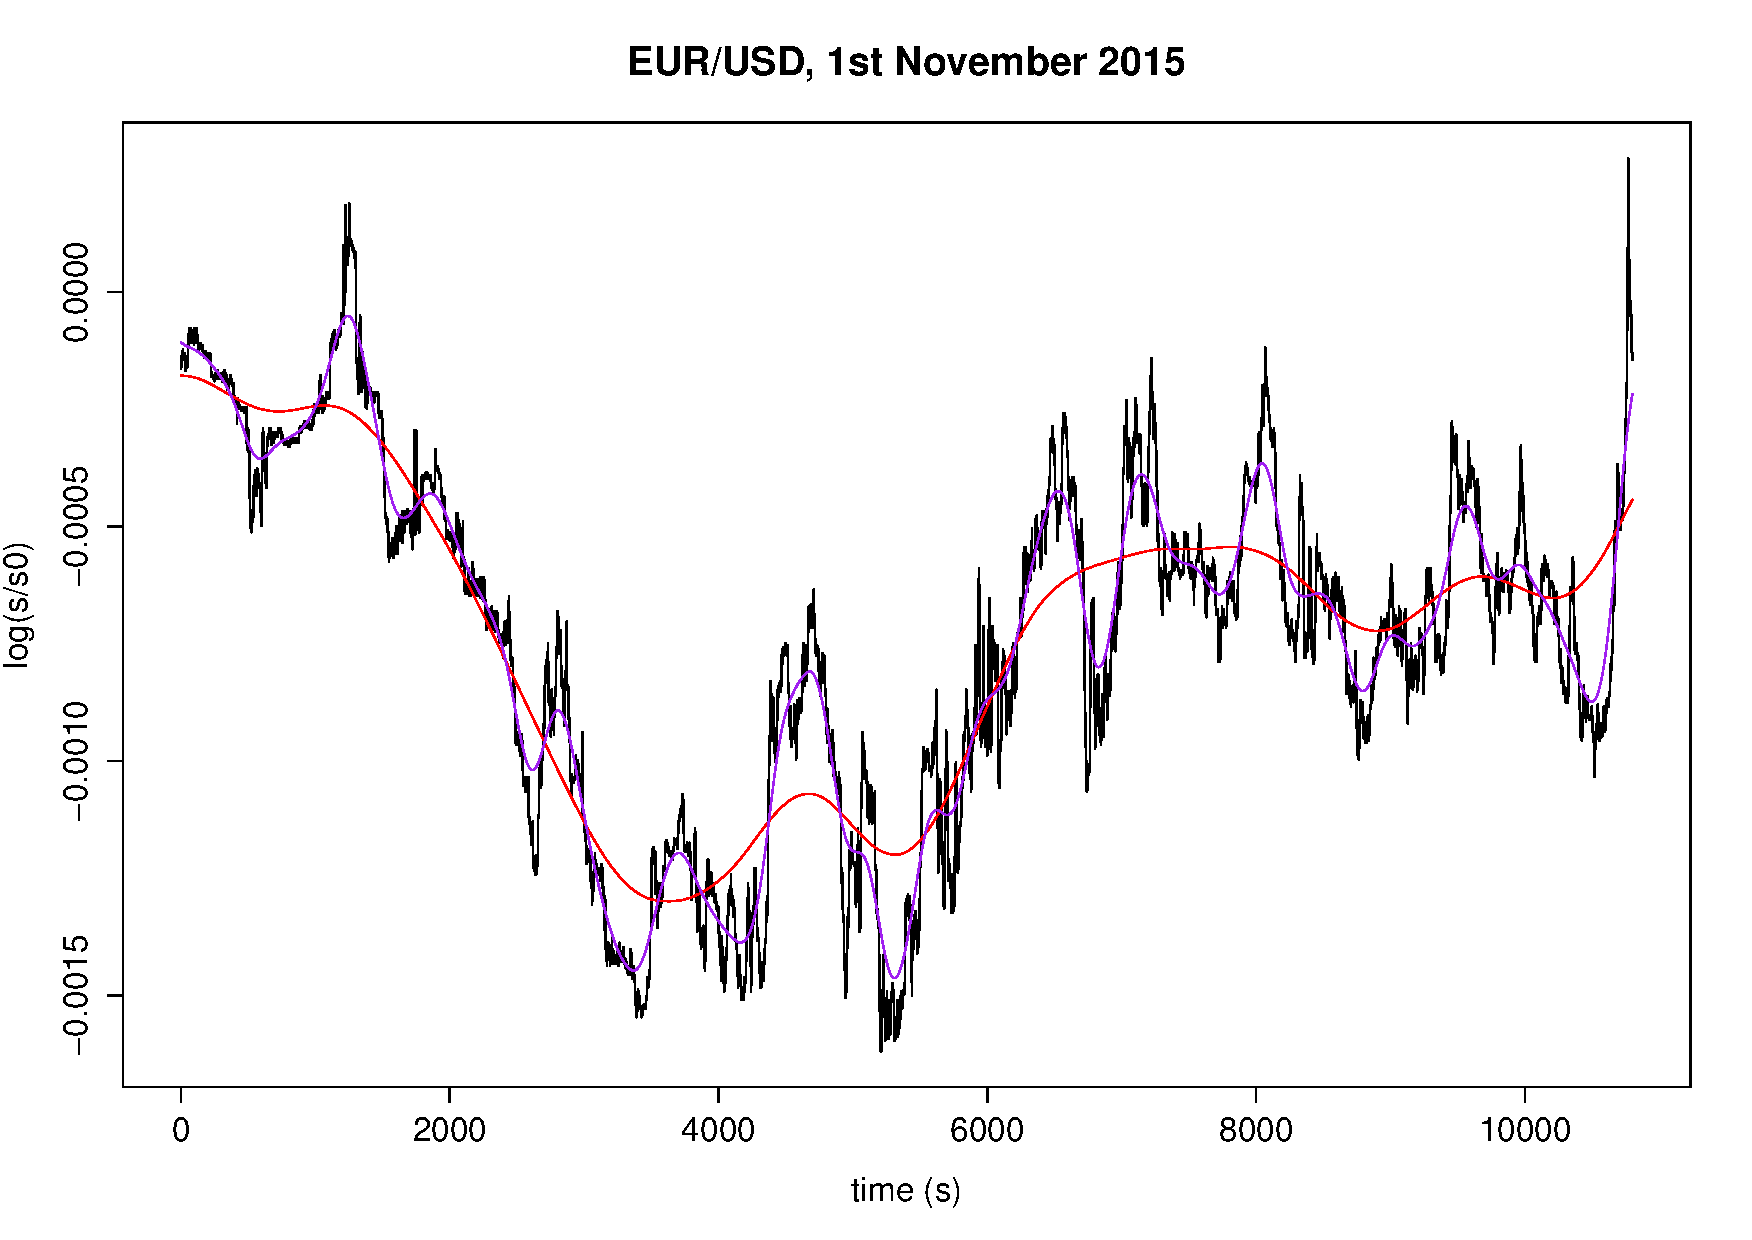
\includegraphics[width=0.6\textwidth,height=0.6\textheight]{figures/asset/ex_filtering}

}
%%%%%%%%%%%%%%%%%%%%%%%%%%%%


%%%%%%%%%%%%%%%%%
\sframe{Génération des données}{
\textbf{Objectif : } Générer $\tilde{X}_i$ tel que avec $\omega_0<\omega_1$,
\begin{enumerate}
\item $\Varb{\tilde{T}_i^{\omega_1}}=\Sigma R$ (covariance contrôlée à plus haute fréquence)
\item  $T_i^{\omega \leq \omega_0} = \tilde{X}_i^{\omega \leq \omega_0}$ (critère de proximité au données)
\end{enumerate}
\medskip
$\mathbf{\rightarrow}$ si $dW_1 \indep dW_1^{\indep}$, alors $W_2 = \rho_{12}W_1 + \sqrt{1-\frac{\sigma_1^2}{\sigma_2^2}\cdot\rho_{12}^2}W_1^{\indep}$ est tel que $\rho(dW_1,dW_2)=\rho_{12}$.

\bigskip

$\rightarrow$ Construction des données par $\tilde{X}_i = T_i^{\omega_0} + W_i - \mathcal{F}_{\omega_0}[W_i]$ avec $\mathcal{F}_{\omega_0}$ filtre passe-bas avec $\omega_c = \omega_0$

}


%%%%%%%%%%%%%%%%%
\sframe{Application}{
$\rightarrow$ \textbf{Signaux :} \emph{log-prix} et \emph{log-retours}, définis par $X(t):=\log{\left(\frac{S(t)}{S_0}\right)}$ et $\Delta X (t) = X(t) - X(t-1)$, pour deux actifs du marché des devises (EUR/USD et EUR/GBP), sur 6 mois de juin 2015 à novembre 2015, filtrés à $\omega_m = 10\textrm{min}$

\bigskip

$\rightarrow$ $\omega_0=24\textrm{h}$ et $\omega_1 = 30\textrm{min},1\textrm{h},2\textrm{h}$

\bigskip

$\rightarrow$ Interférence entre différentes échelles
\[
\rho_e \simeq \left[ \varepsilon_1 \varepsilon_2 \rho_0 + \rho \right] \cdot \left[ 1 - \frac{1}{2}\left(\varepsilon_1^2 + \varepsilon_2^2 \right) \right]
\]


}



%%%%%%%%%%%%%%%%%
\sframe{Résultats : Correlations effectives}{

\textit{Correlations simulées et correlations théoriques à différentes fréquences}

\centering
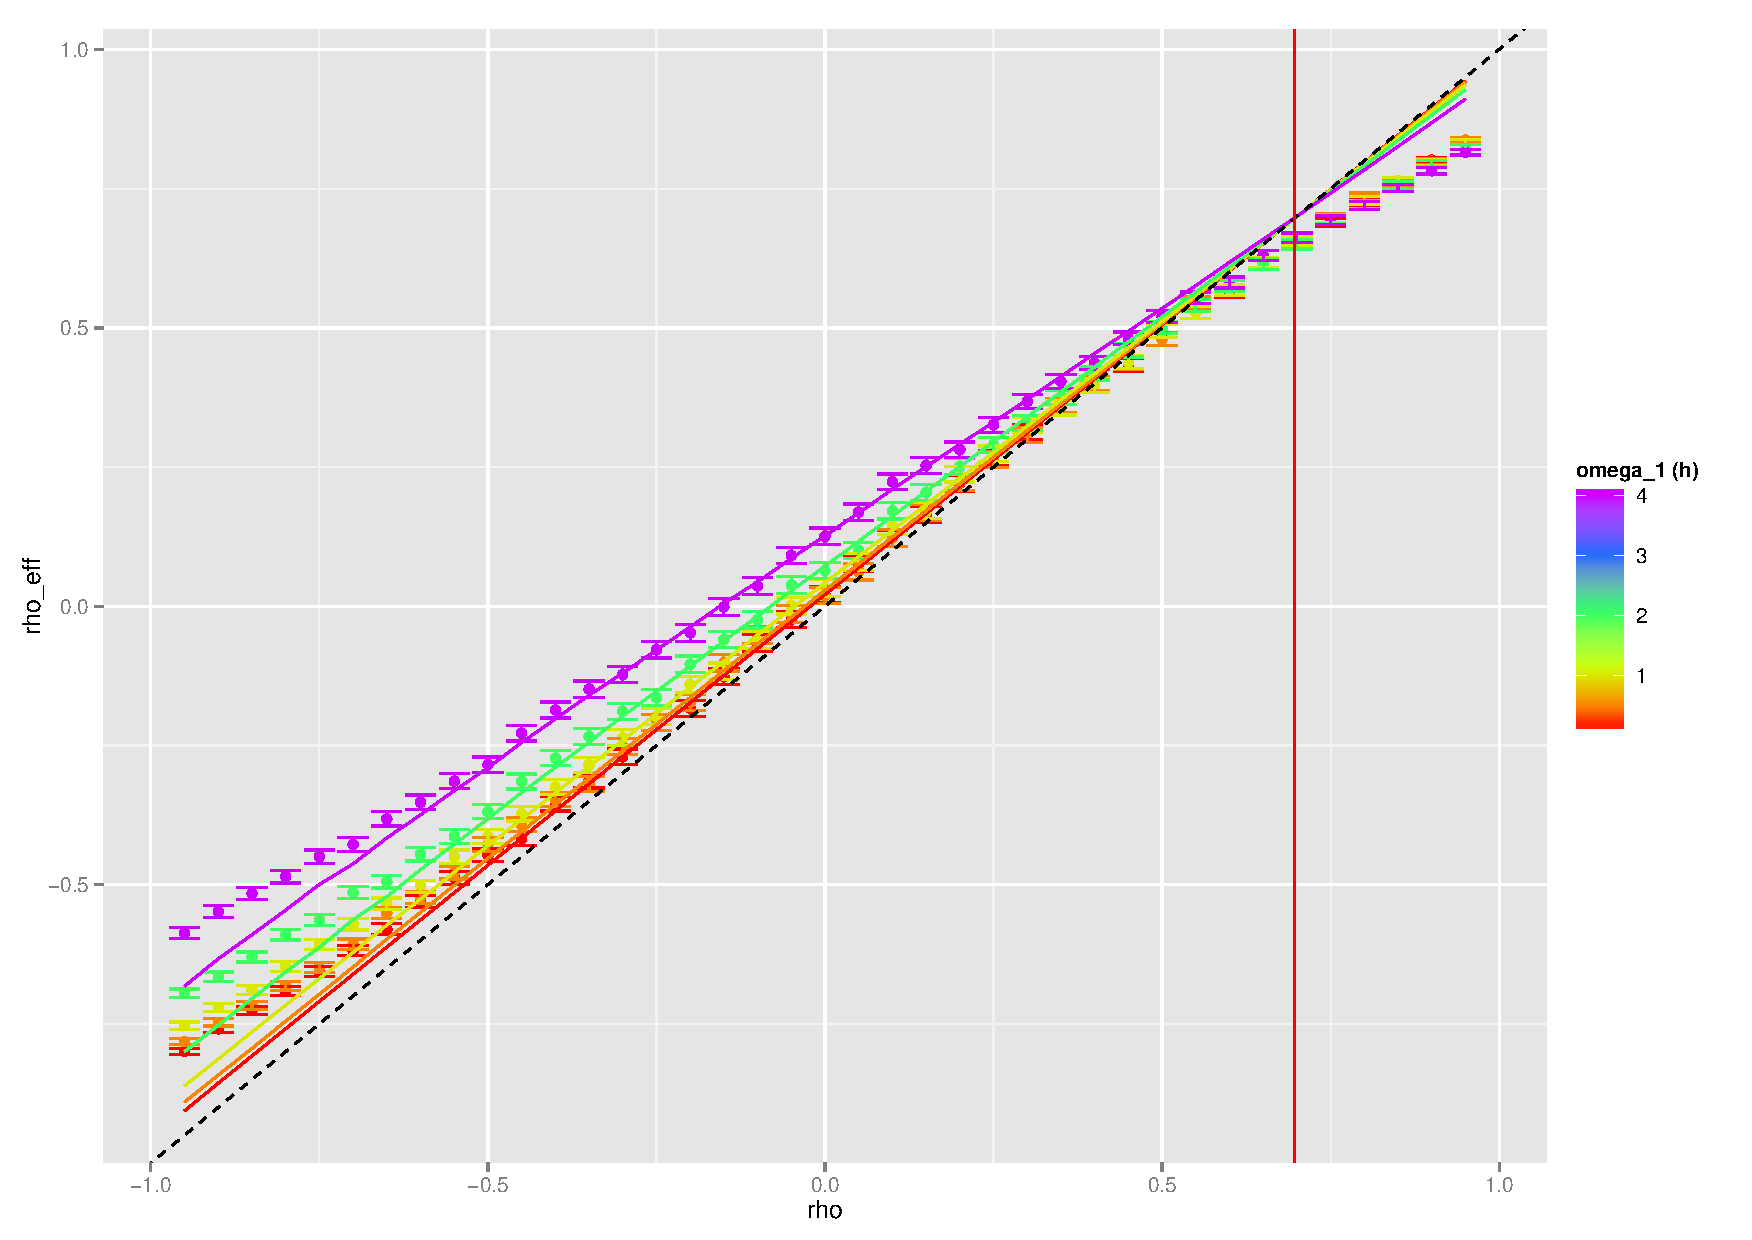
\includegraphics[width=0.8\textwidth,height=0.8\textheight]{figures/effectiveCorrs_withGoodTh_A4}

}

%%%%%%%%%%%%%%%%%
\sframe{Résultats : Performance d'un modèle prédictif}{
\centering
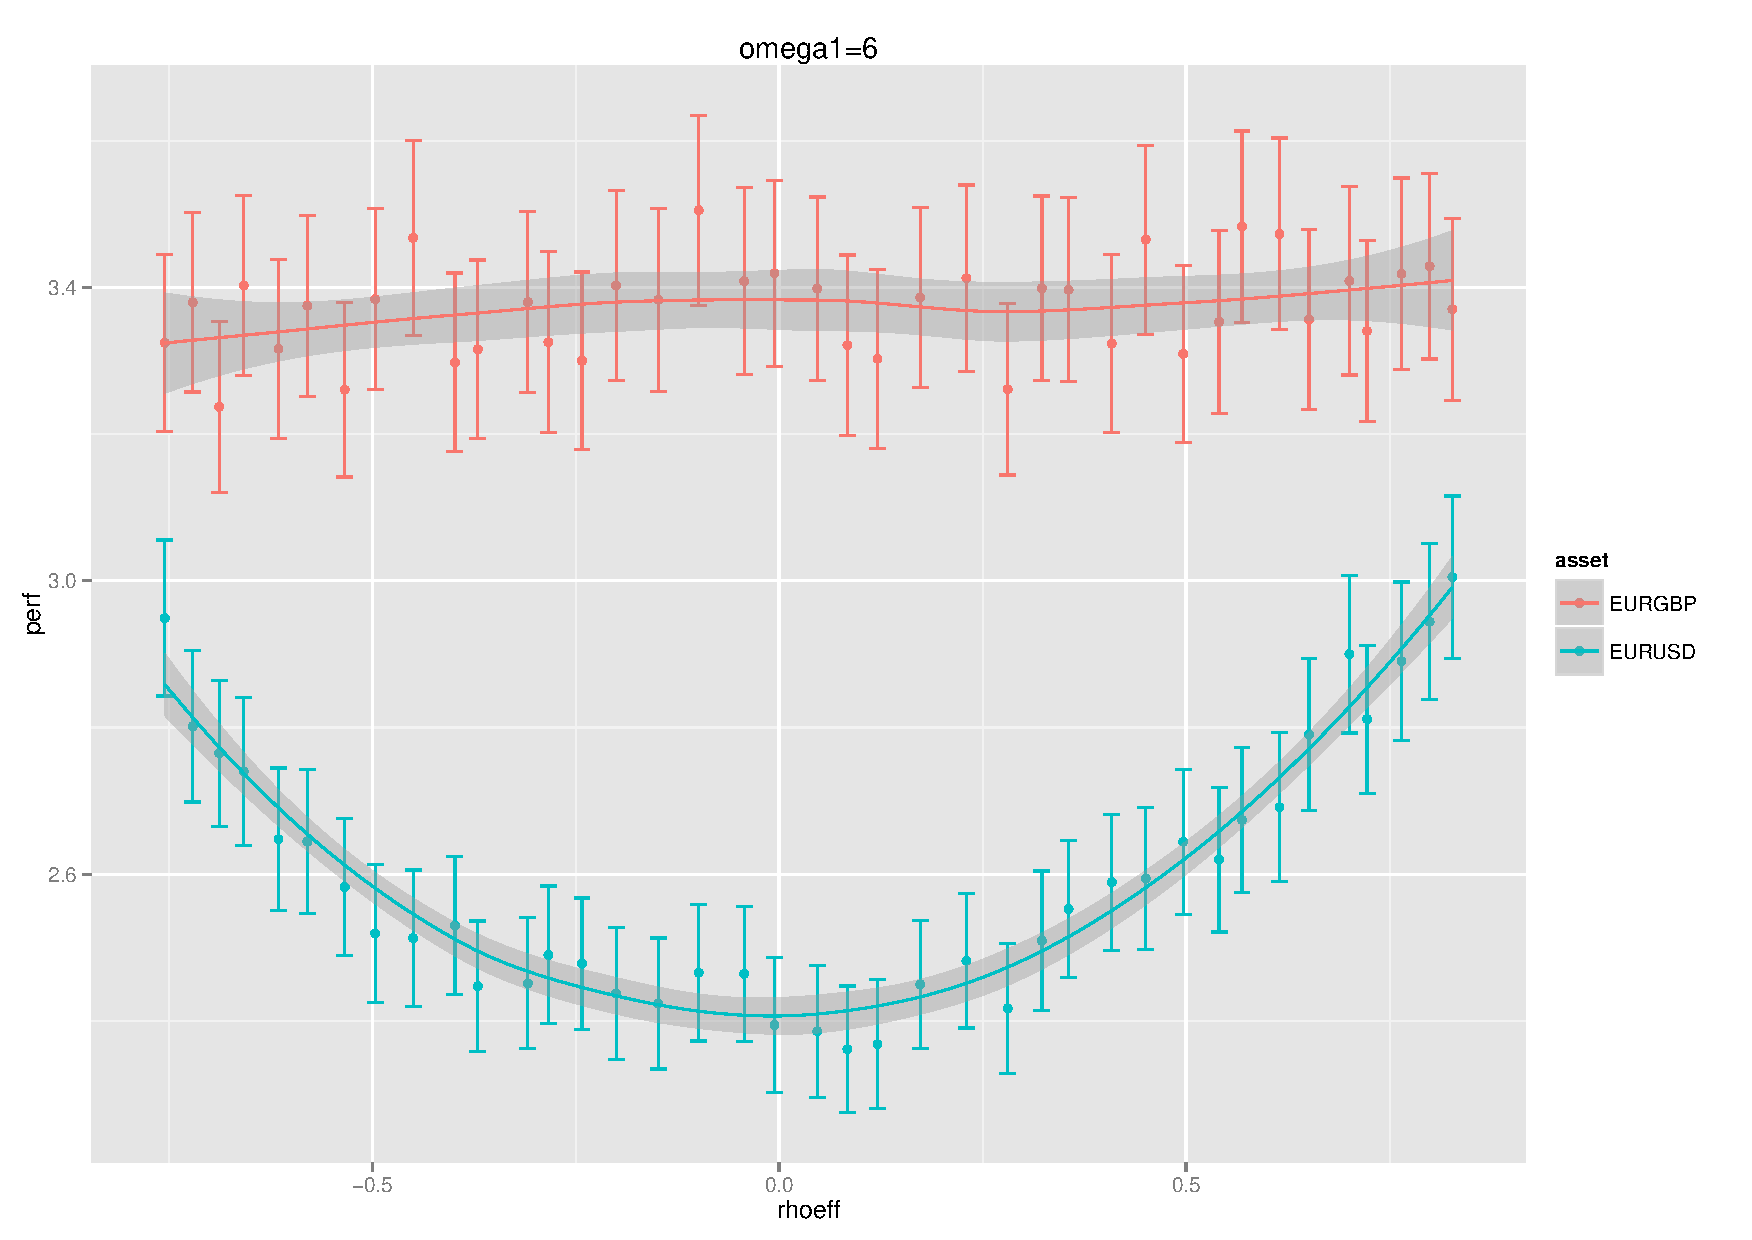
\includegraphics[width=0.48\textwidth,height=0.45\textheight]{figures/asset/pred_filt6}
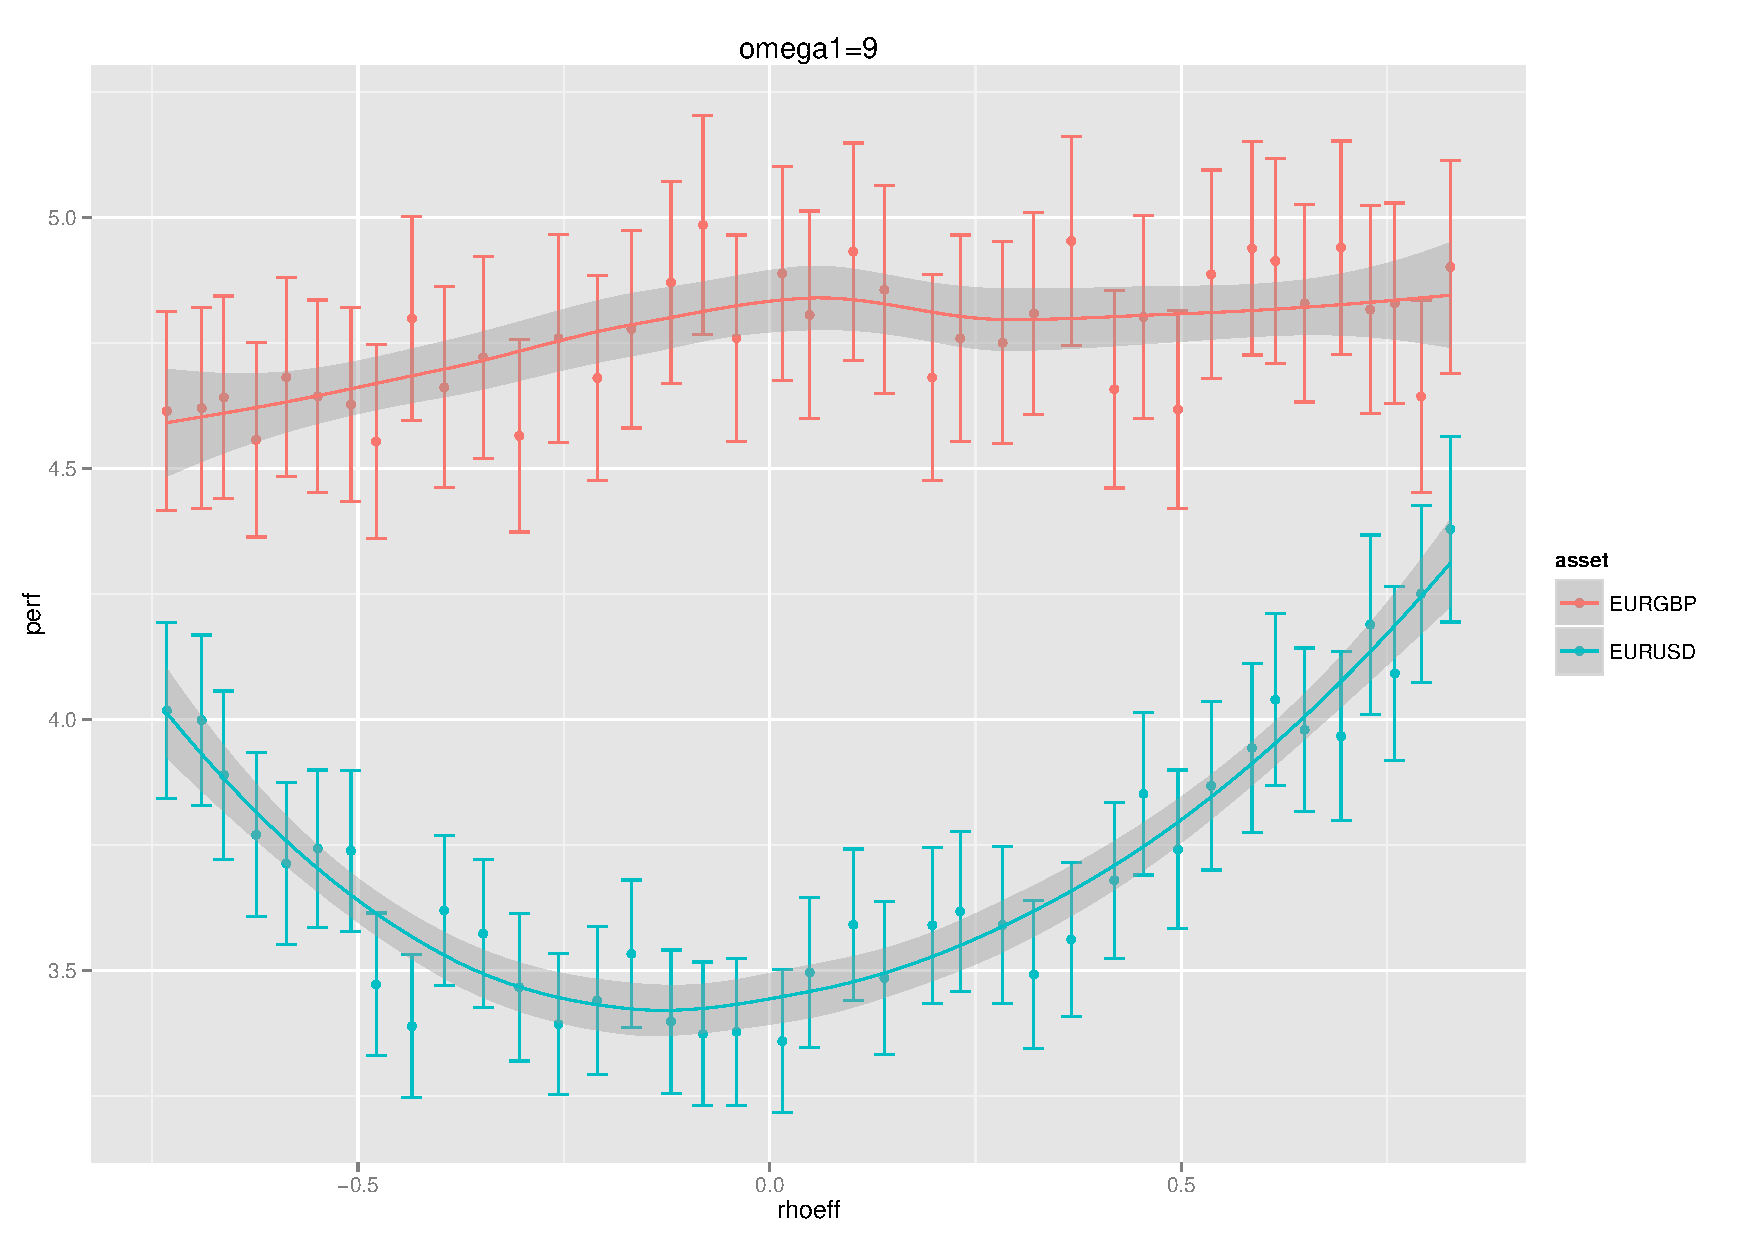
\includegraphics[width=0.48\textwidth,height=0.45\textheight]{figures/asset/pred_filt9}\\
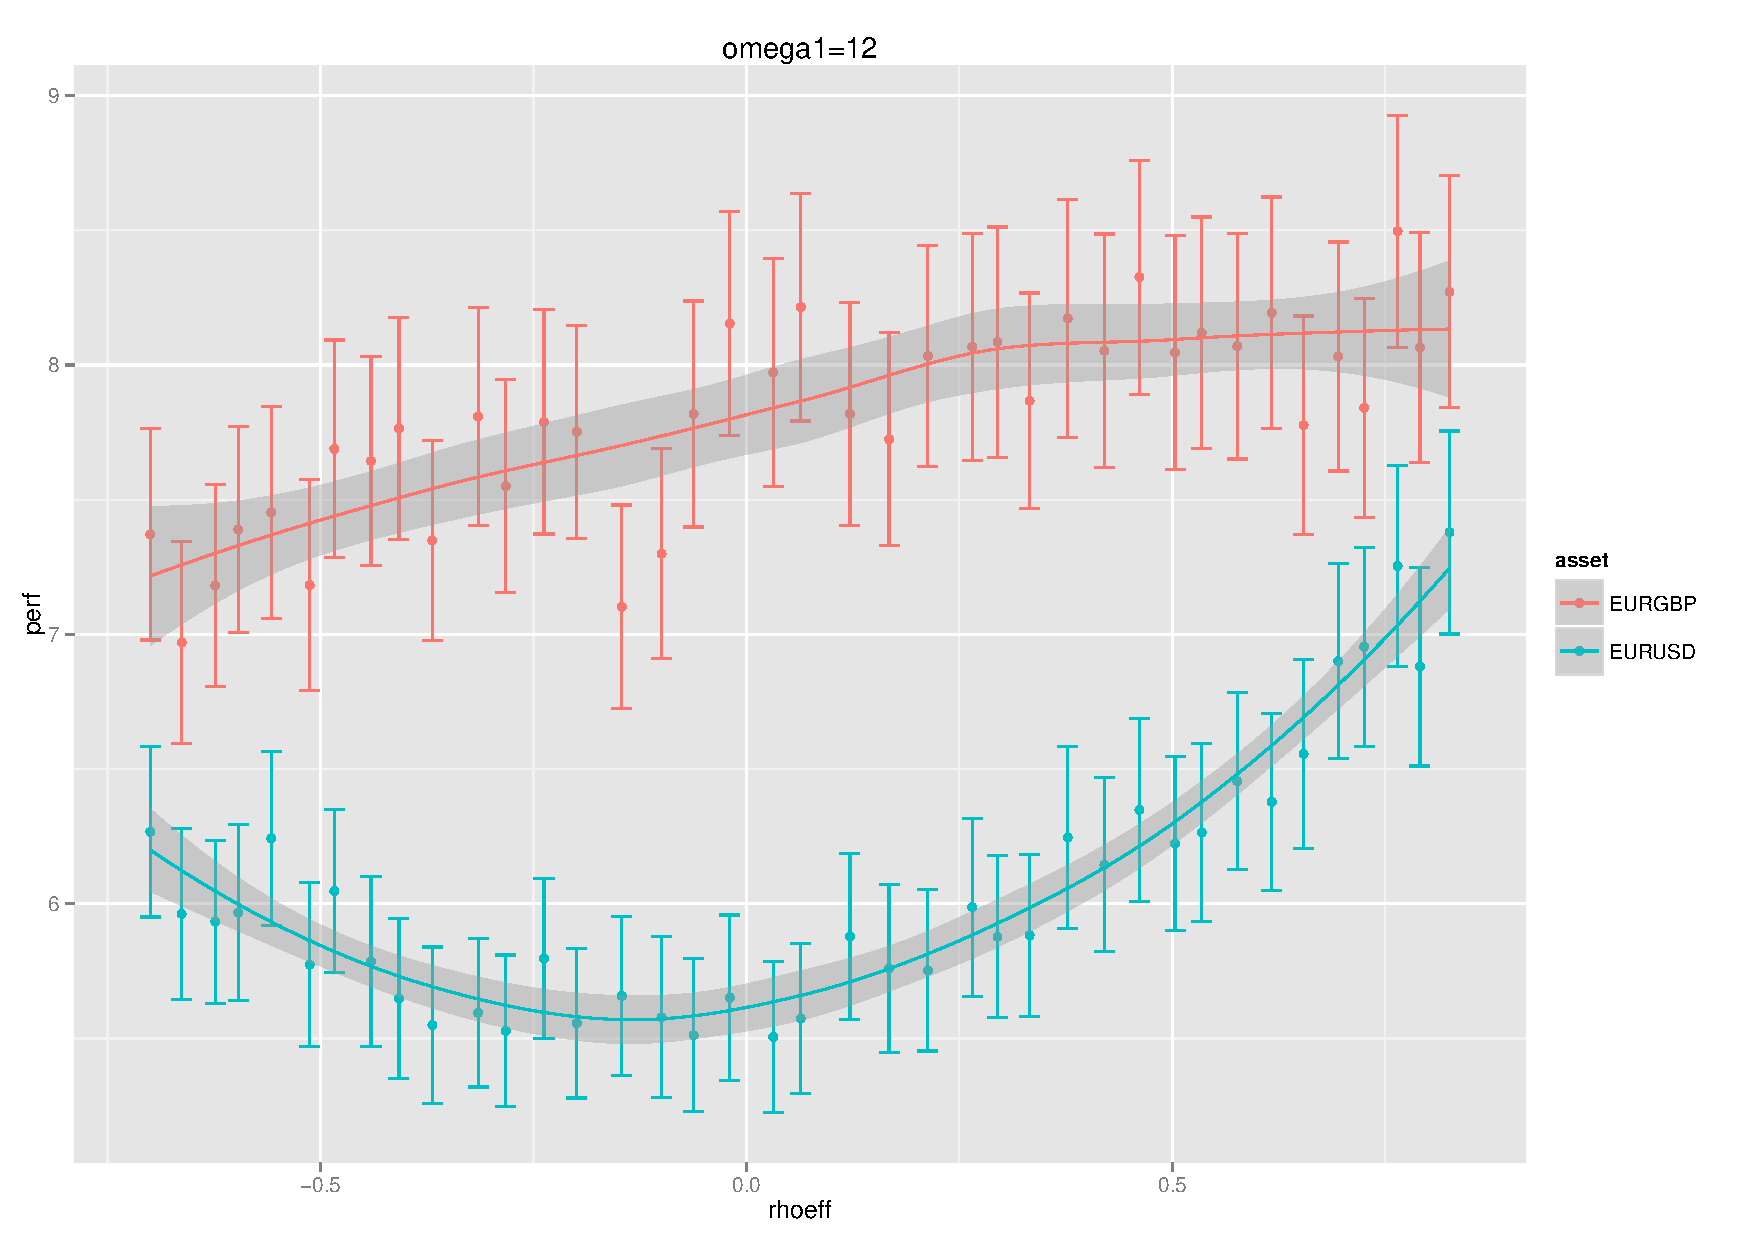
\includegraphics[width=0.48\textwidth,height=0.45\textheight]{figures/asset/pred_filt12}
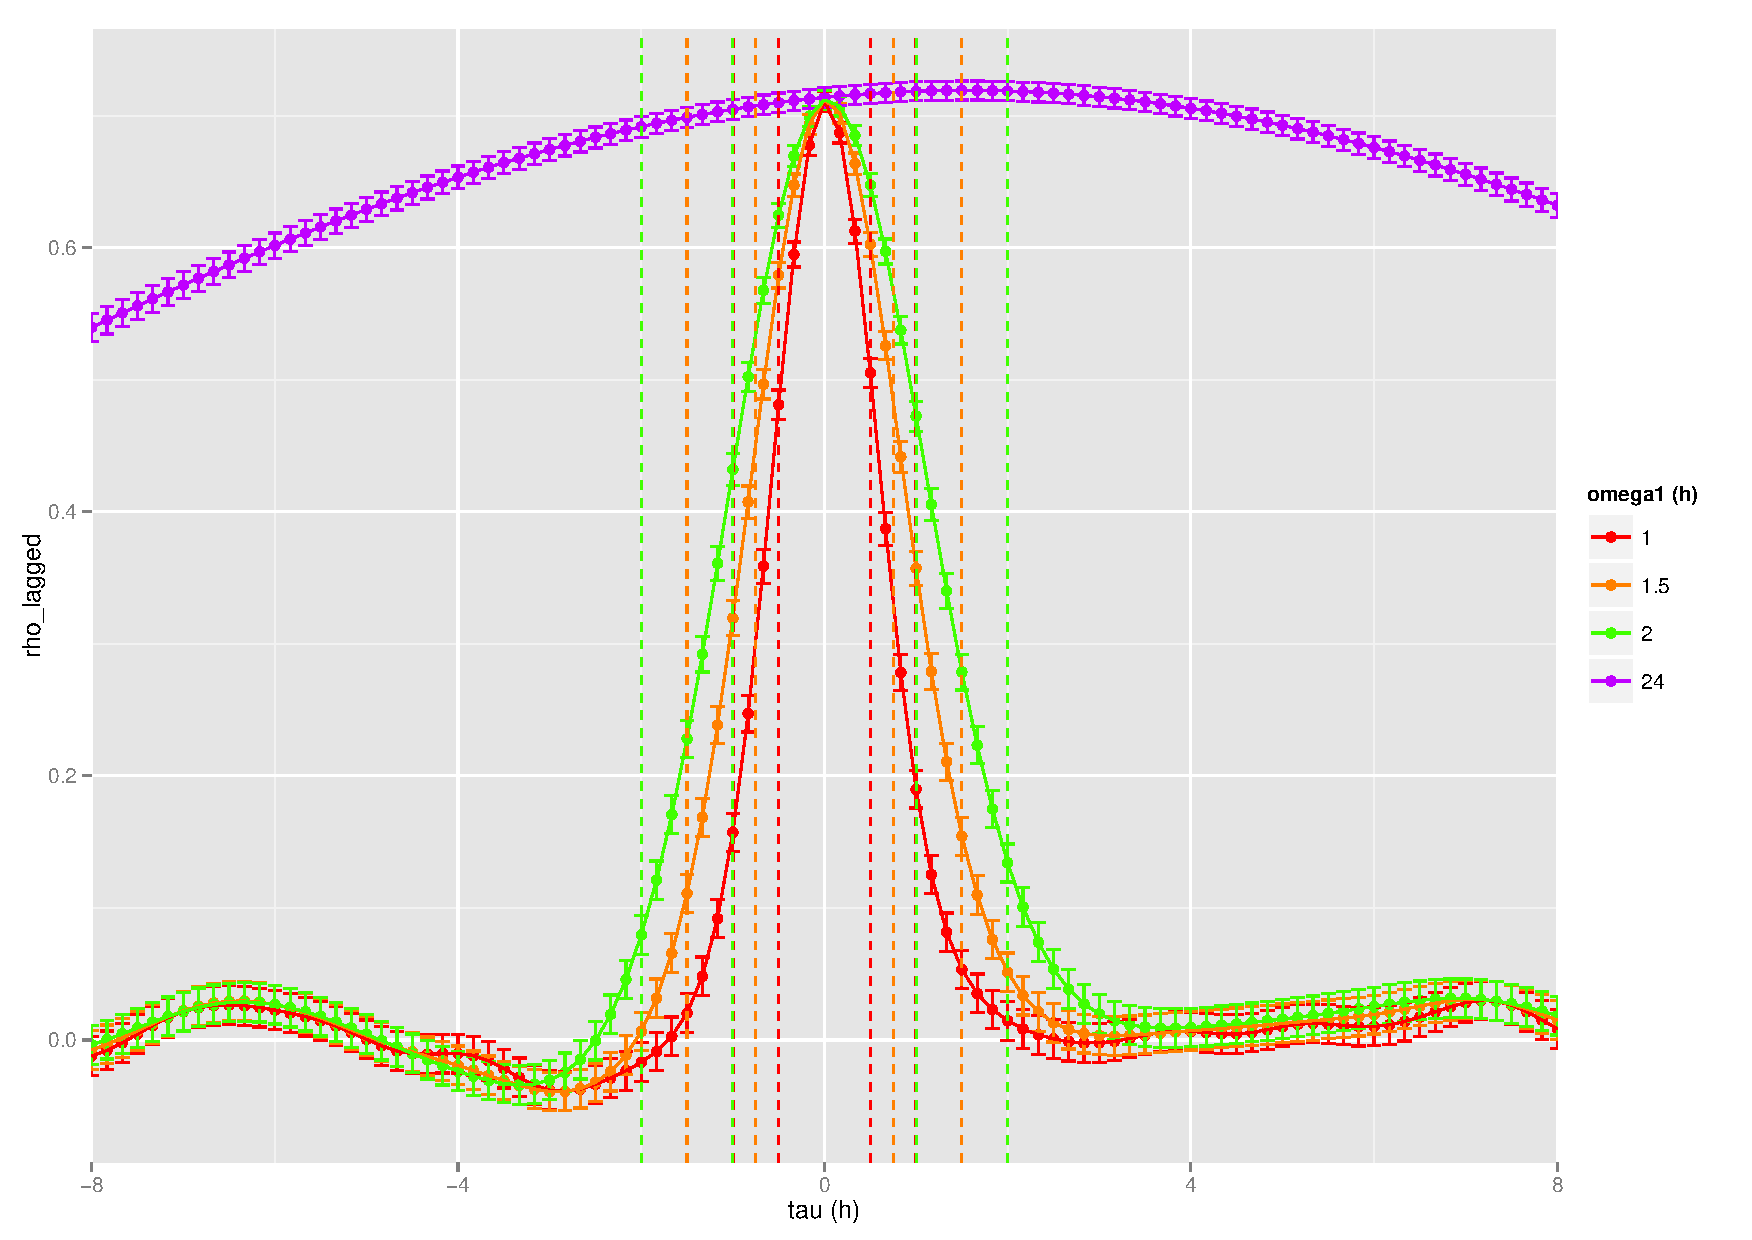
\includegraphics[width=0.48\textwidth,height=0.45\textheight]{figures/asset/lagged_corrs}
}



%%%%%%%%%%%%%%%%%
\subsection{Données géographiques}
%%%%%%%%%%%%%%%%%

%%%%%%%%%%%%%%%%%
\sframe{Données géographiques : Contexte et Objectif}{

\begin{itemize}
\jitem{En géographie, génération de population synthétiques pour modèles agents~\cite{pritchard2009advances}.}
\jitem{Génération de configurations spatiales synthétiques peu répandue (Régression Géo. Pondérée~\cite{brunsdon1998geographically} peut être interprétée de cette façon) ; pourtant essentielle même pour des modèles abstraits~\cite{schmitt2014modelisation}}
\jitem{\cite{cottineau2015revisiting} a récemment proposé d'estimer la sensibilité des modèles de simulation spatiaux à la configuration spatiale initiale (application au modèle de Schelling).}
\jitem{Cas d'étude : relations ville/transports, complexe à cerner quantitativement~\cite{offner1993effets,bretagnolle:tel-00459720} $\rightarrow$ modèle simple de morphogénèse de densité de population et de réseau de transport.}
\end{itemize}
}



%%%%%%%%%%%%%%%%%
\sframe{Modèle}{
\footnotesize
Couplage simple entre
\begin{itemize}
\jitem{Génération itérative d'une grille de densité par attachement préférentiel/diffusion \cite{raimbault2016calibration}, calibrée sur objectifs morphologiques sur grille européenne de densité.}
\jitem{Génération heuristique de réseau conditionnelle à la densité :
\begin{itemize}
\footnotesize
\item Distribution d'un nombre fixé de centres par attachement préférentiel selon la distribution de densité
\item Percolation déterministe par plus proche voisins
\item Rupture des potentiels d'interaction
\[
V_{ij}(d) = \left[ (1 - k_h) + k_h \cdot \left( \frac{P_i P_j}{P^2} \right)^{\gamma} \right]\cdot \exp{\left( -\frac{d}{r_g (1 + d/d_0)} \right)}
\]
pour un nombre fixé de couples $N_L$ tels que $V_{ij}(d_N)/V_{ij}(d_{ij})$ est minimal parmi $K\cdot N_L$ plus forts potentiels euclidiens ($K=5$ fixé)
\item Planarification
\end{itemize}
}
\end{itemize}
Indicateurs : morphologie~\cite{le2015forme} (Moran, distance moyenne, entropie, hiérarchie) et réseau (centralité, largeur moyenne, vitesse, diamètre).

}

%%%%%%%%%%%%%%%%%
\sframe{Implémentation et exploration}{

$\rightarrow$ Couplage formel et opérationnel : implémentation modulaire (\texttt{scala}/\texttt{NetLogo}) encapsulée par \texttt{OpenMole}~\cite{reuillon2013openmole}

\bigskip

$\rightarrow$ Exploration par calcul intensif sur grille de calcul via \texttt{OpenMole} : calibration du modèle de densité seul sur grille de densité européenne ($\sim 1.5\cdot 10^6$ runs) ; exploration brute par criblage LHS pour corrélations faisables ($\sim 5\cdot 10^4$ runs) 

}



%%%%%%%%%%%%%%%%%
\sframe{Résultats : Modèle de densité seul}{
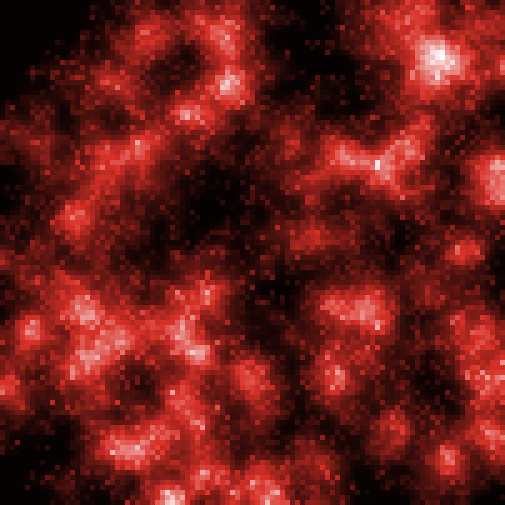
\includegraphics[width=0.24\textwidth]{figures/density/conf1}\hspace{0.1em}
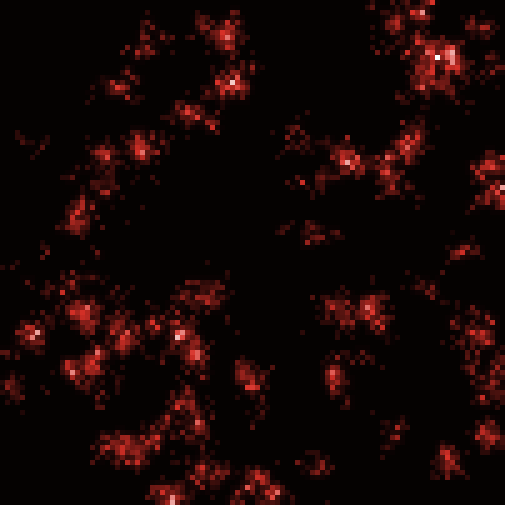
\includegraphics[width=0.24\textwidth]{figures/density/conf2}\hspace{0.1em}
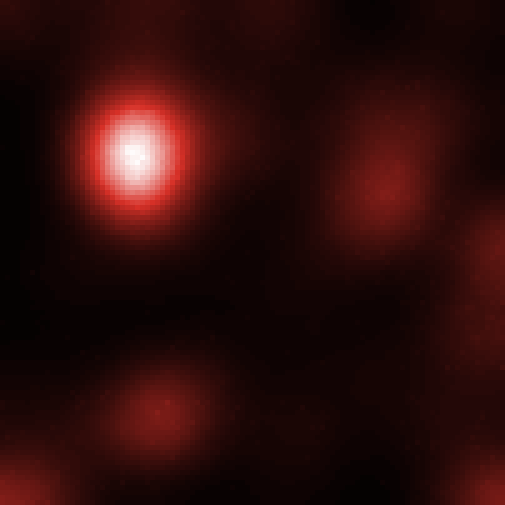
\includegraphics[width=0.24\textwidth]{figures/density/conf3}\hspace{0.1em}
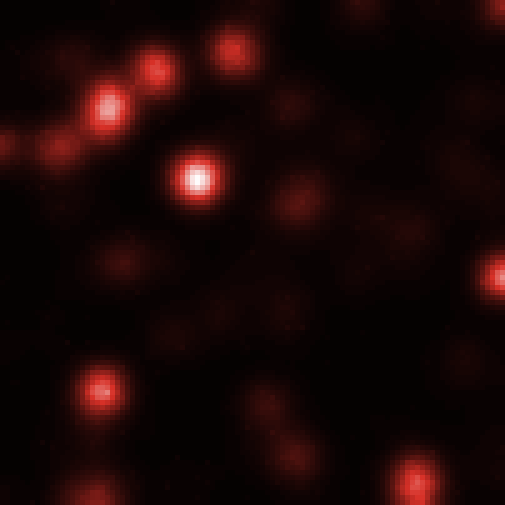
\includegraphics[width=0.24\textwidth]{figures/density/conf4}\hspace{0.1em}
\\
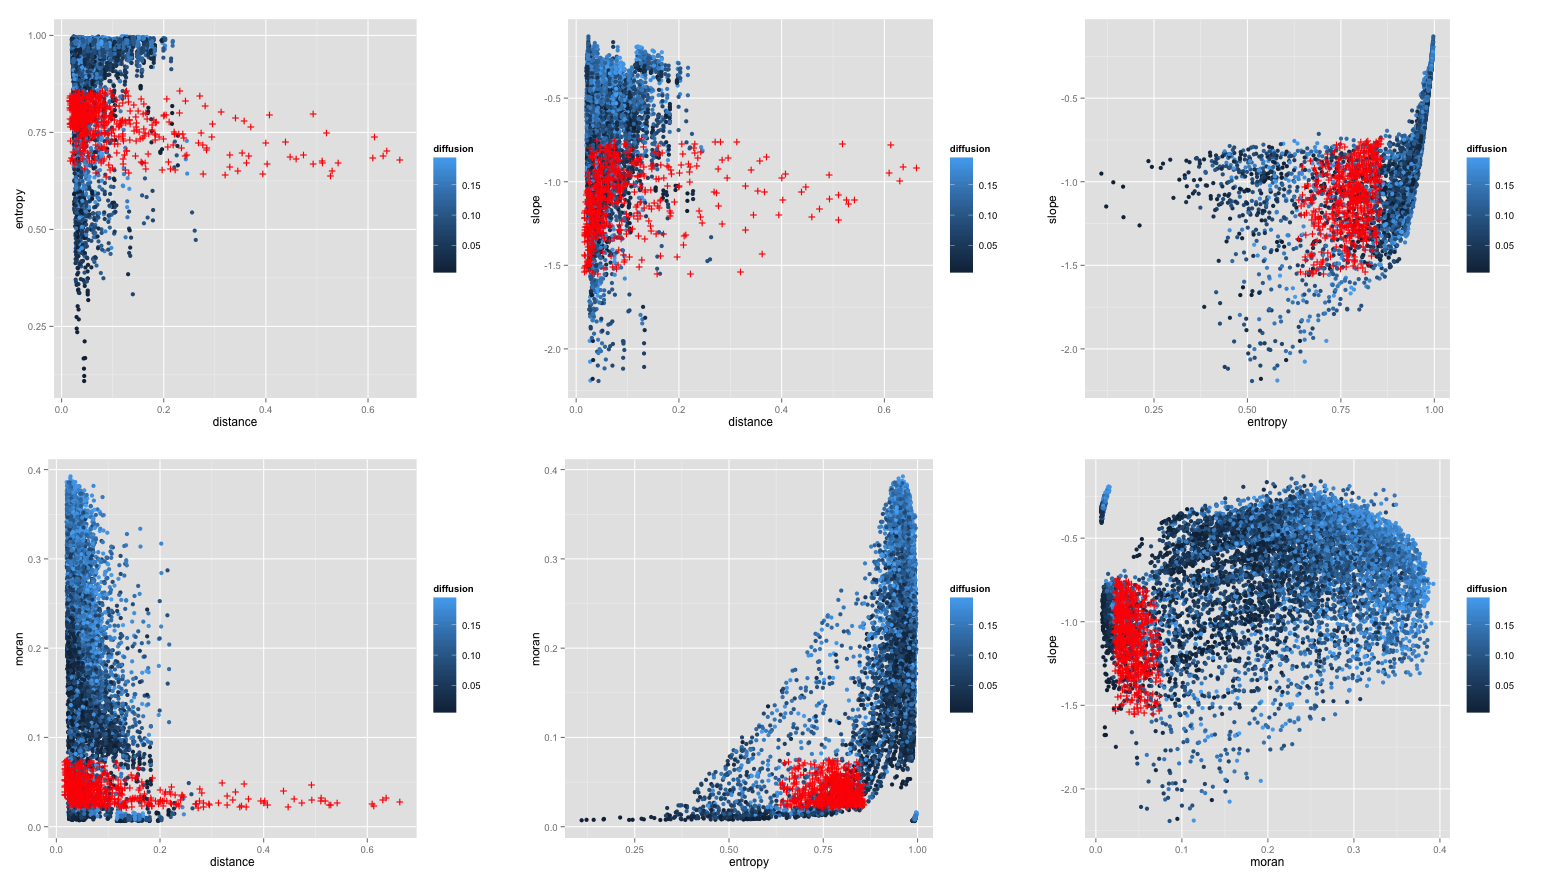
\includegraphics[width=0.5\textwidth,height=0.55\textheight]{figures/density/scatt}
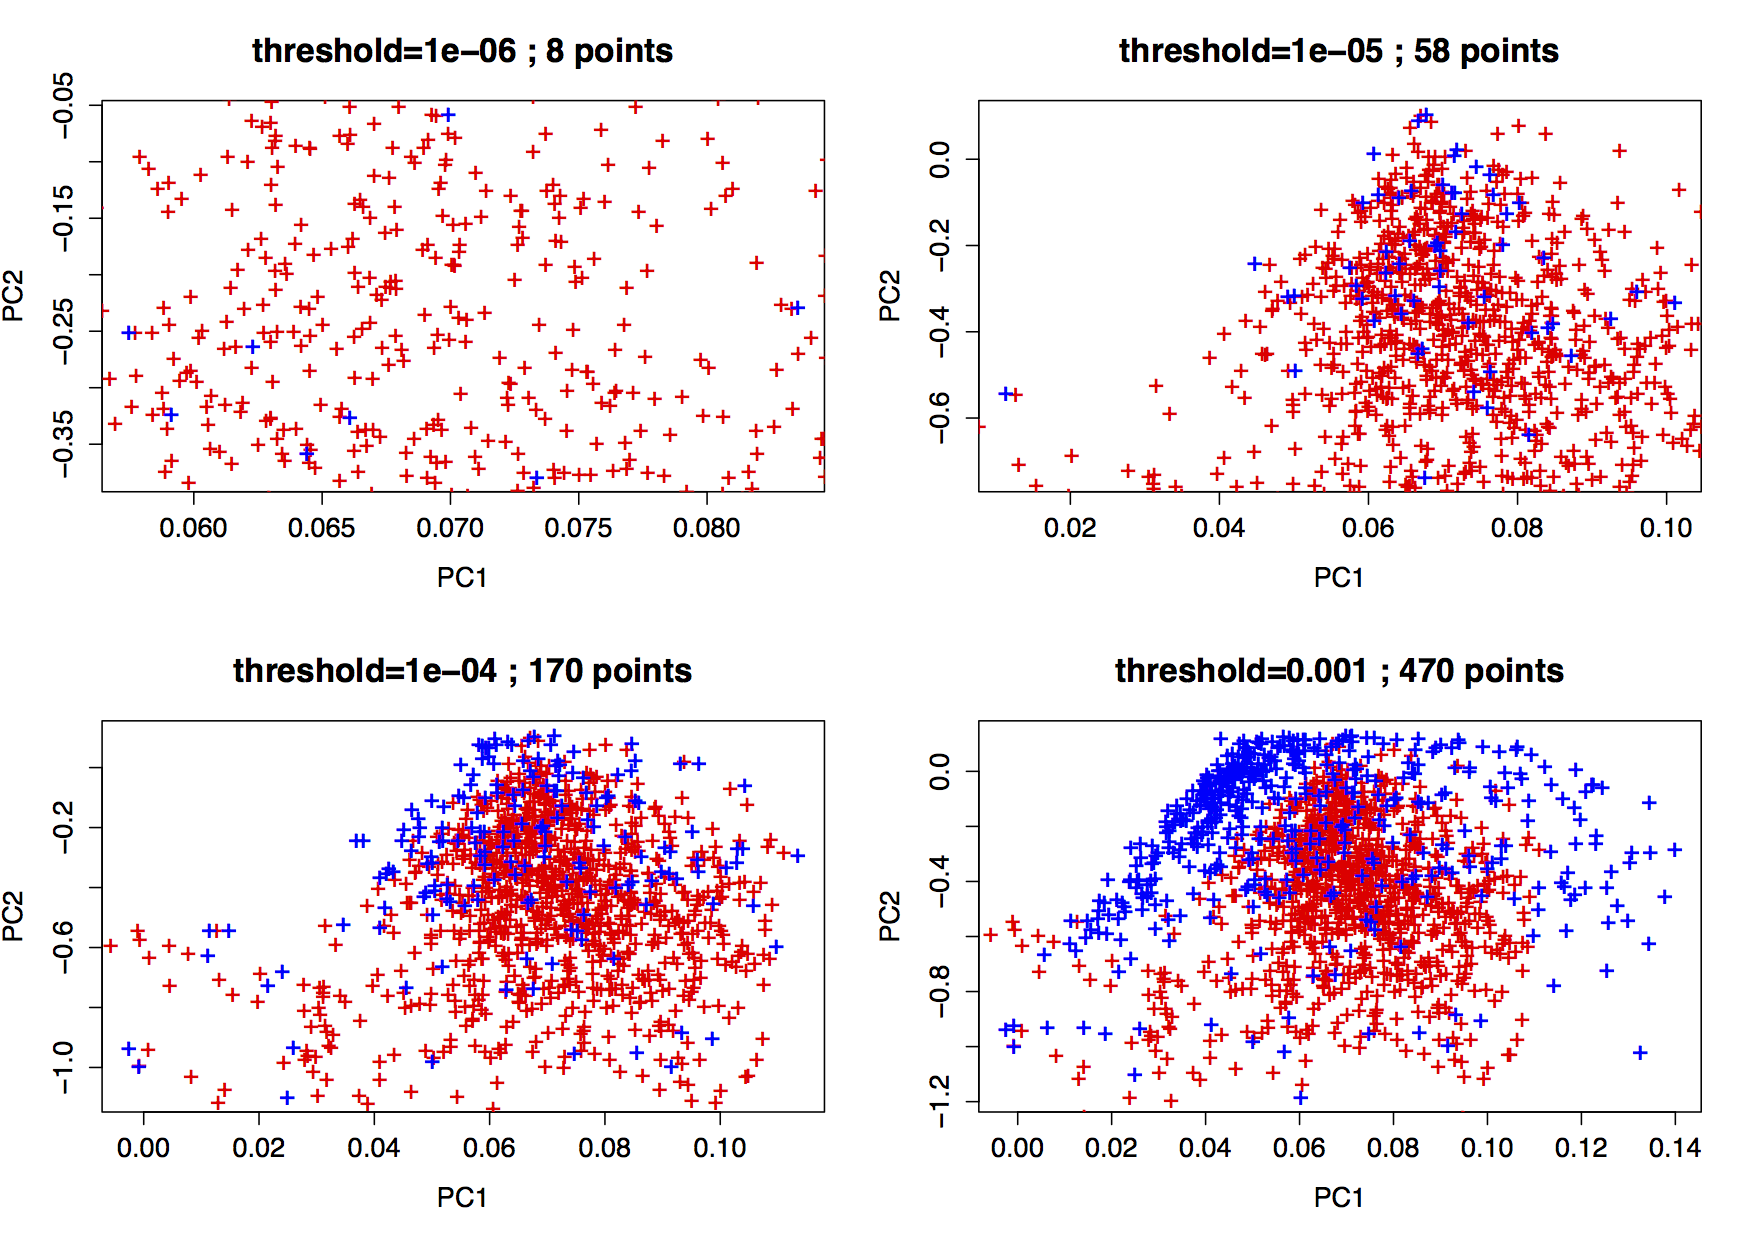
\includegraphics[width=0.5\textwidth,height=0.55\textheight]{figures/density/pca}
}



%%%%%%%%%%%%%%%%%
\sframe{Résultats : exemples de configurations}{
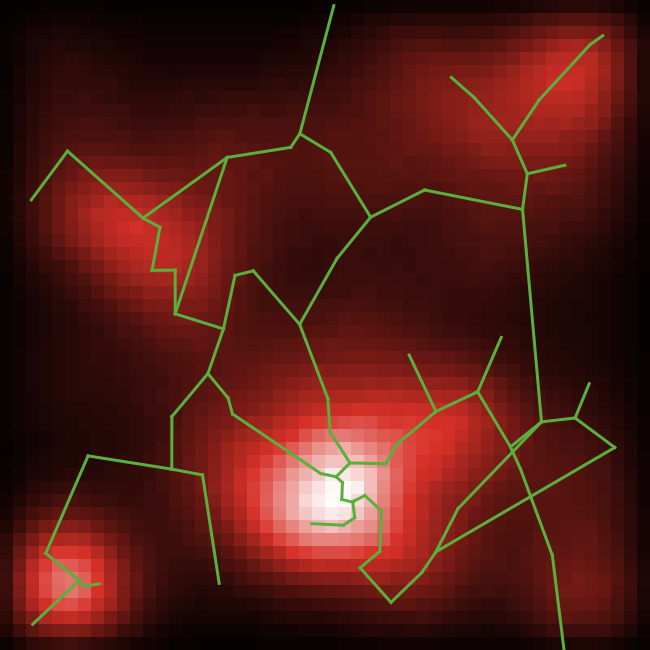
\includegraphics[width=0.49\textwidth]{figures/configs/2_param71913_seed10}\hspace{0.1cm}
   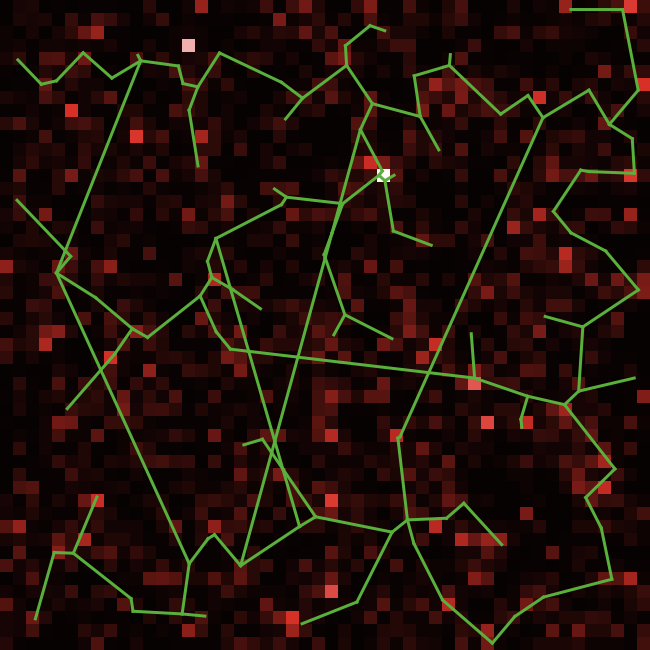
\includegraphics[width=0.49\textwidth]{figures/configs/3_param71918_seed0}
}

%%%%%%%%%%%%%%%%%
\sframe{Résultats : exemples de configurations}{
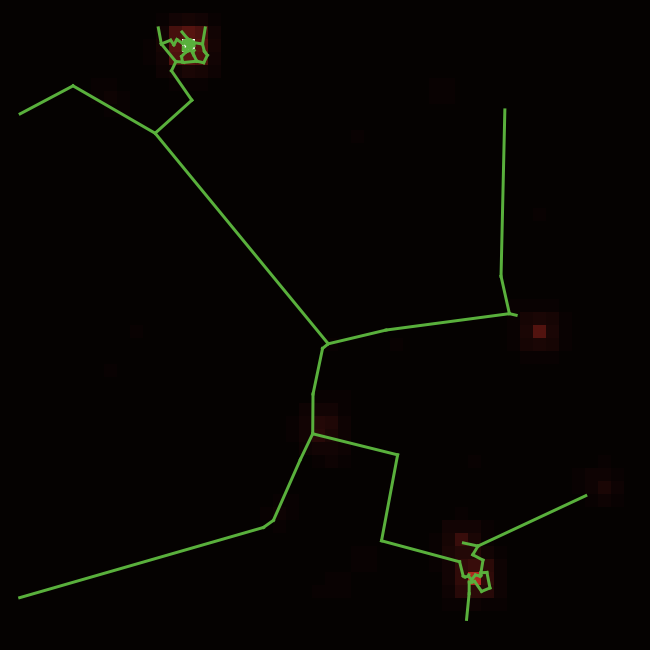
\includegraphics[width=0.49\textwidth]{figures/configs/1_param71861_seed0}\hspace{0.1cm}
   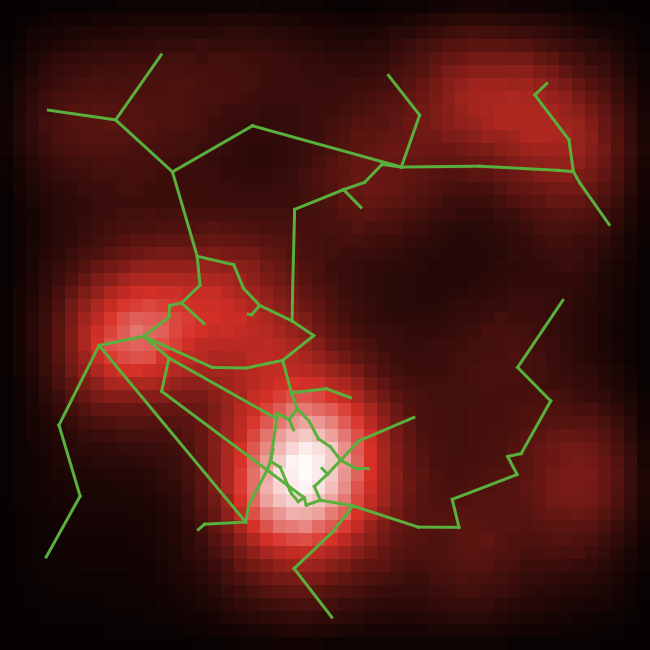
\includegraphics[width=0.49\textwidth]{figures/configs/4_param71945_seed0}
}




%%%%%%%%%%%%%%%%%
\sframe{Résultats : corrélations croisées}{
\centering
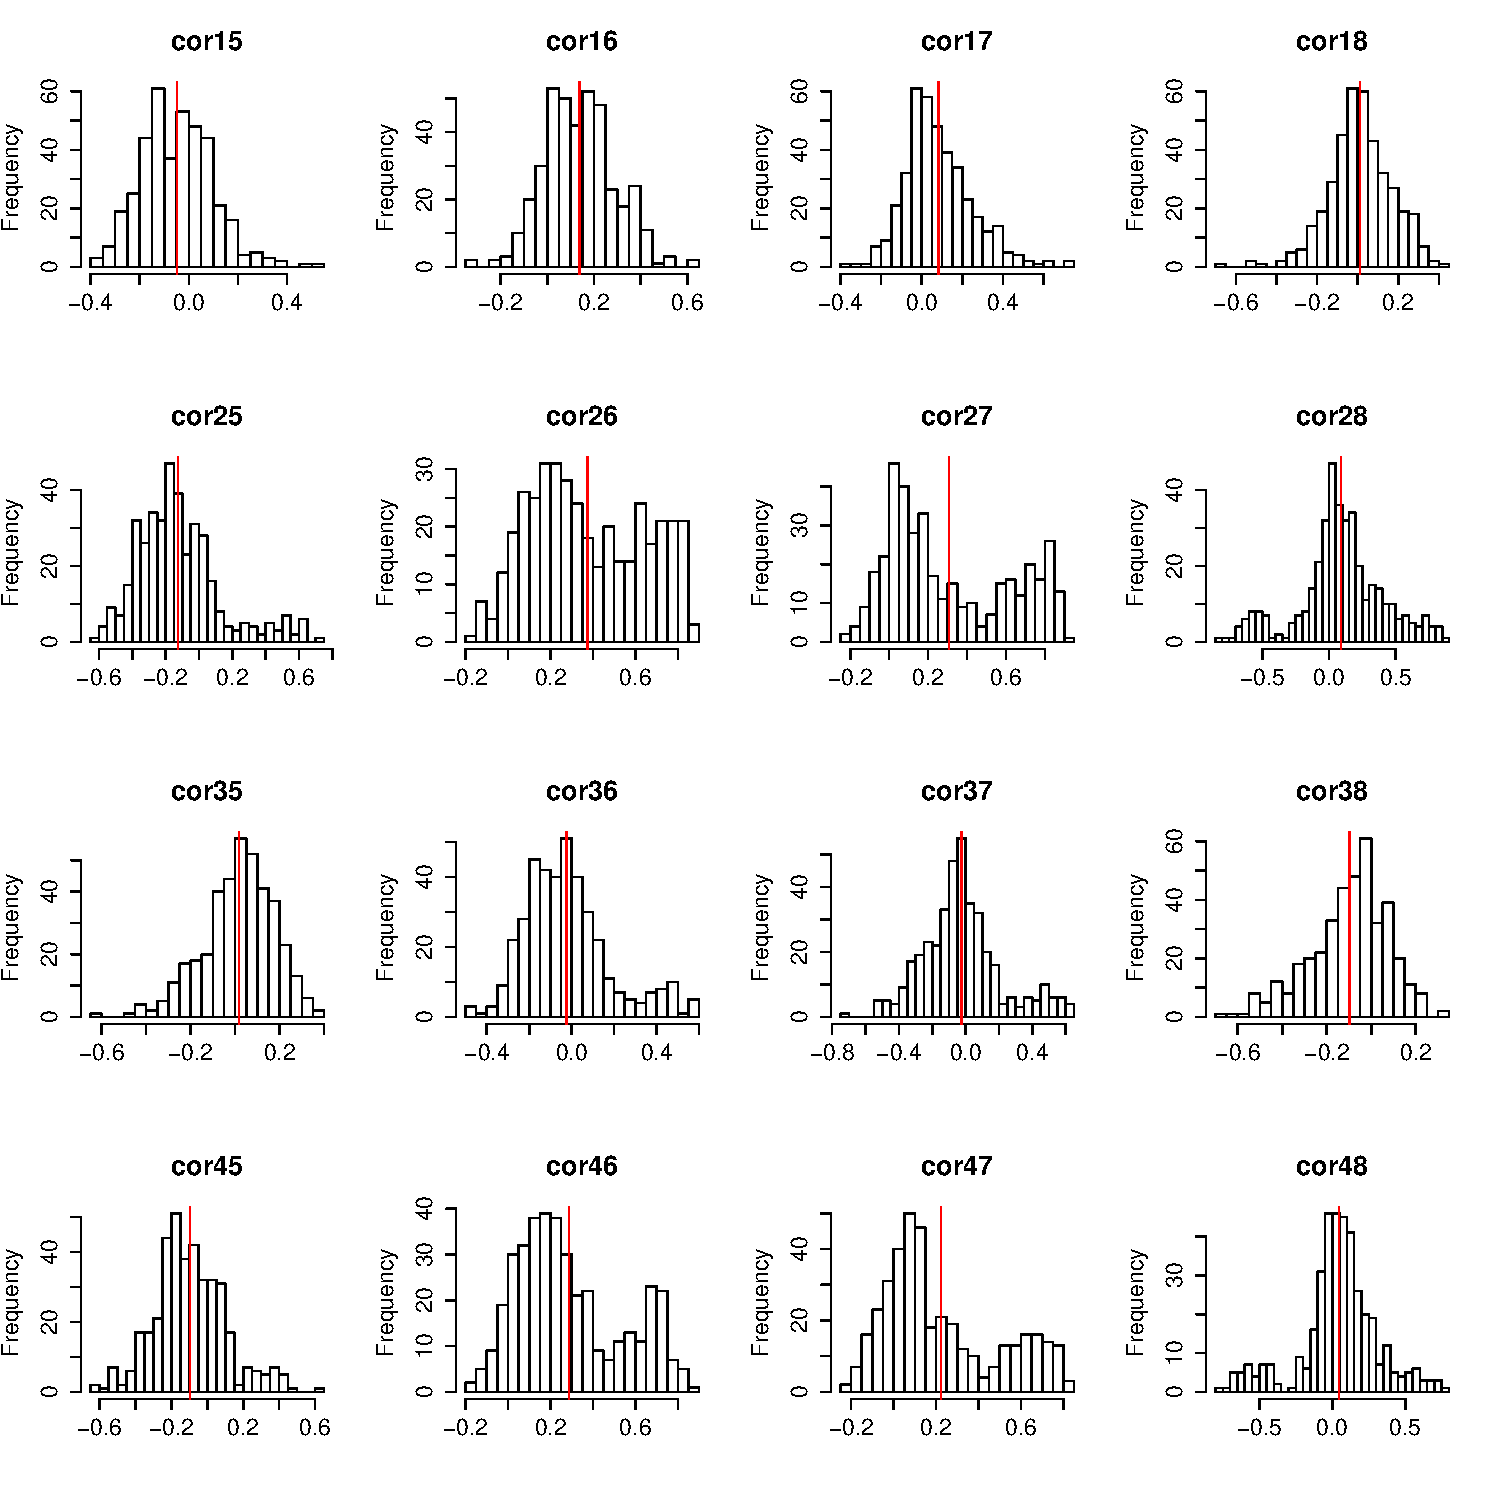
\includegraphics[height=0.85\textheight]{figures/hist_crossCorMat_breaks30}
}

%%%%%%%%%%%%%%%%%
\sframe{Résultats : corrélations faisables}{
\textit{Matrices moyennes dans un plan principal}
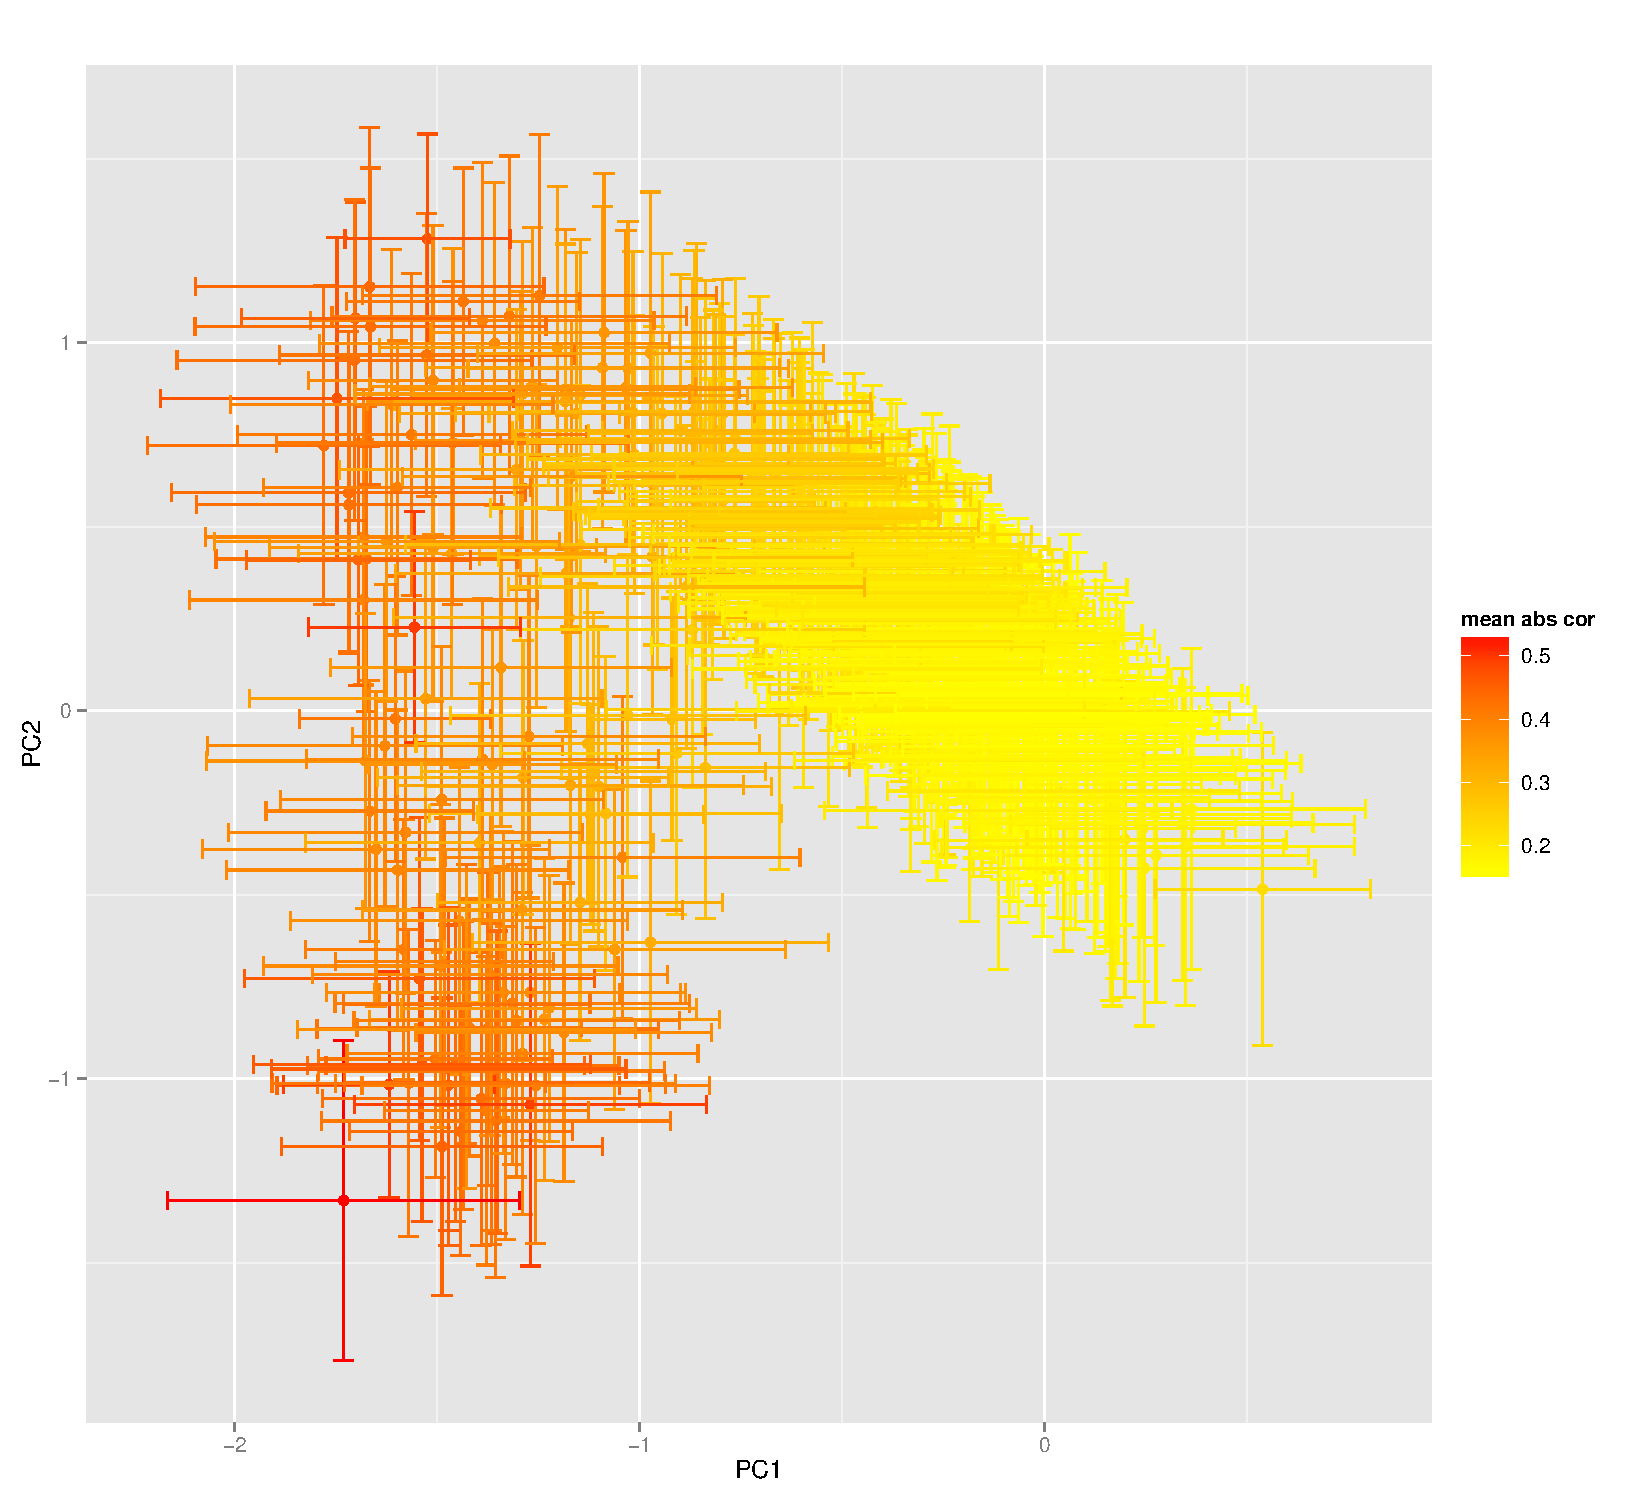
\includegraphics[width=0.5\textwidth,height=0.7\textheight]{figures/pca_meanAbsCor_errorBars}
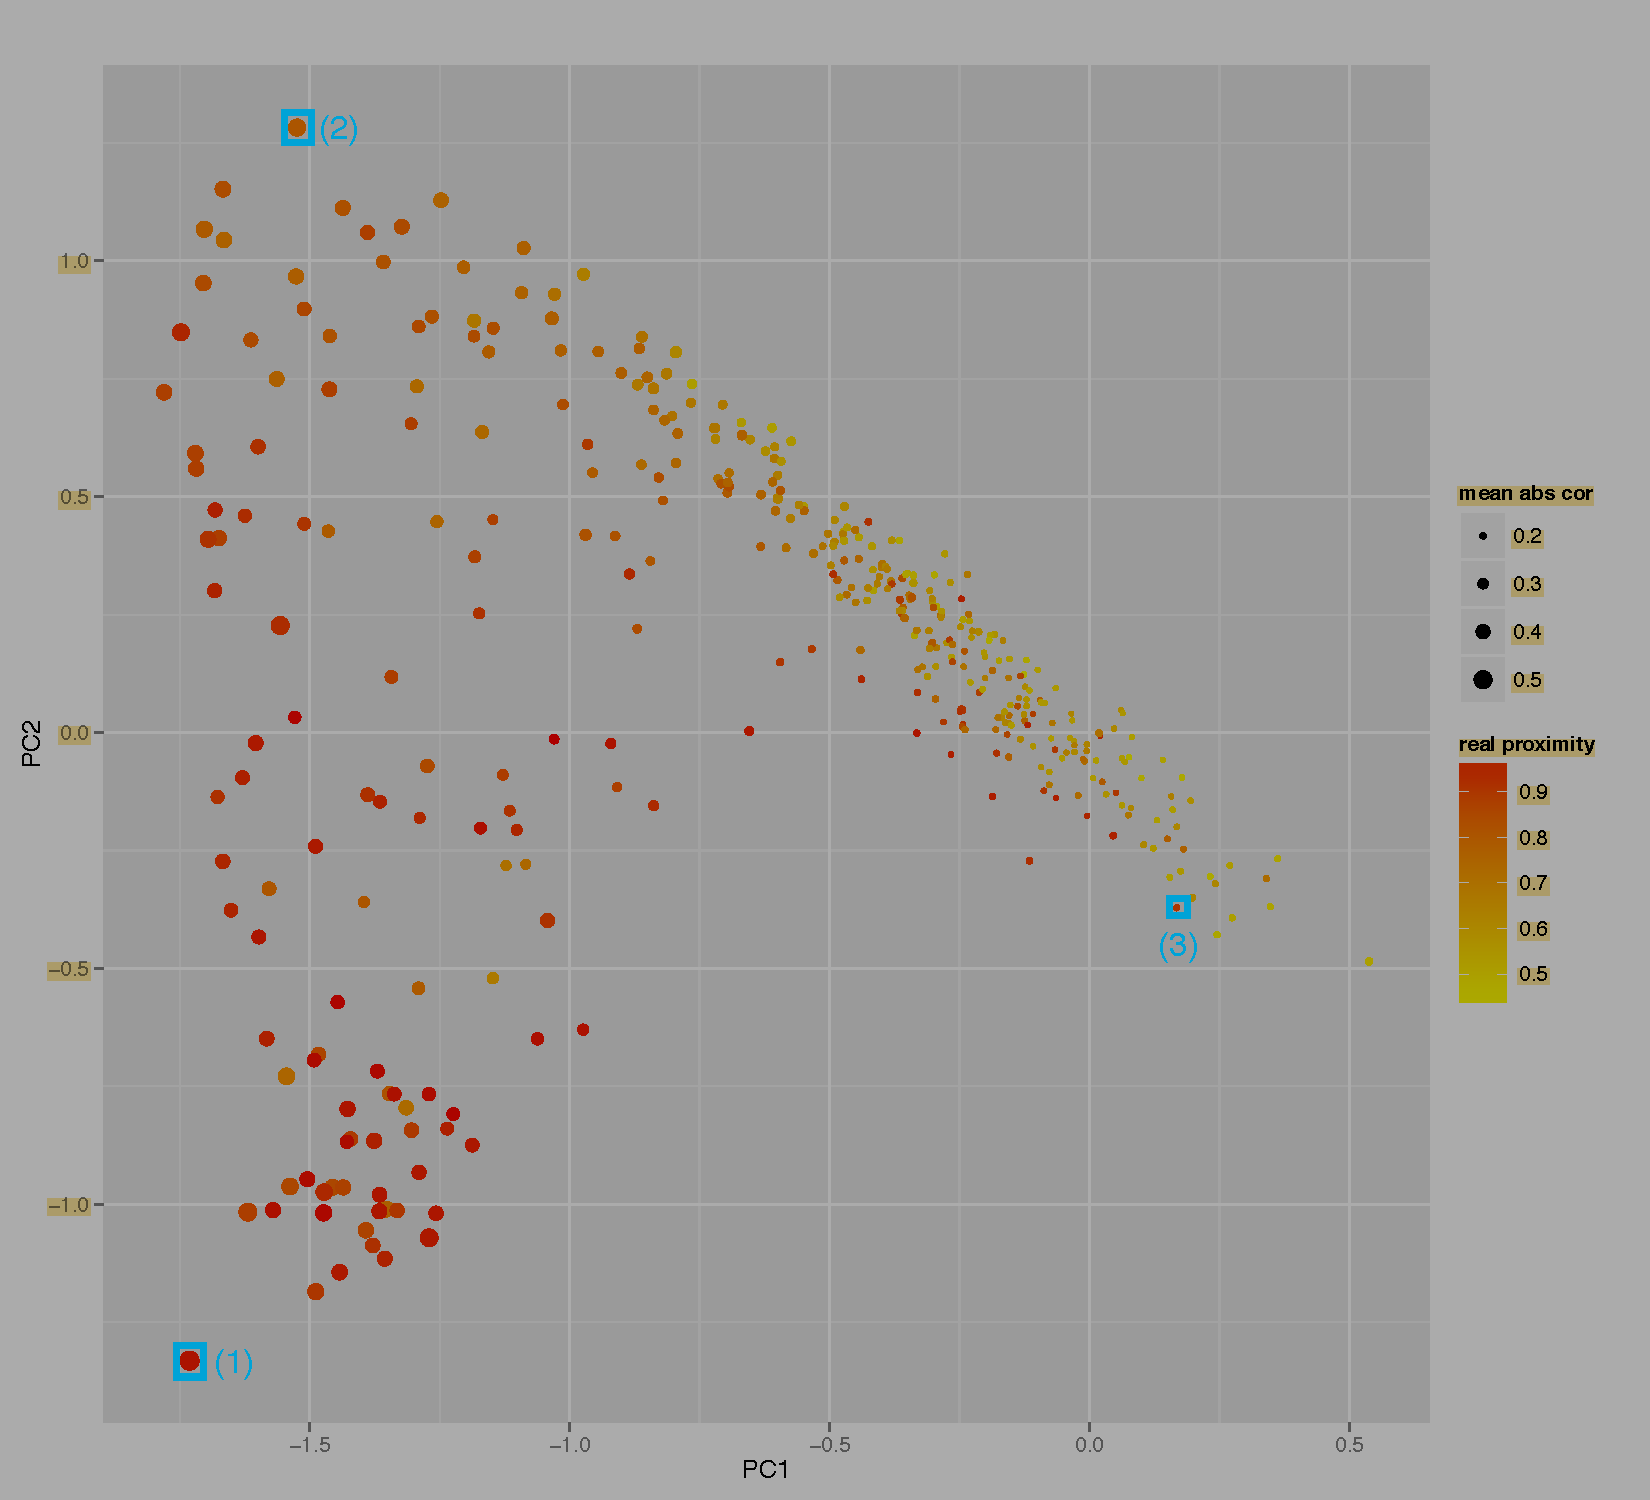
\includegraphics[width=0.5\textwidth,height=0.7\textheight]{figures/pca_realDistCol_meanAbsCorSize_withSpecificPoints}
}

%%%%%%%%%%%%%%%%%
\sframe{Résultats : exemples de correlations}{
\begin{columns}[T] % align columns
\begin{column}{.48\textwidth}
\centering
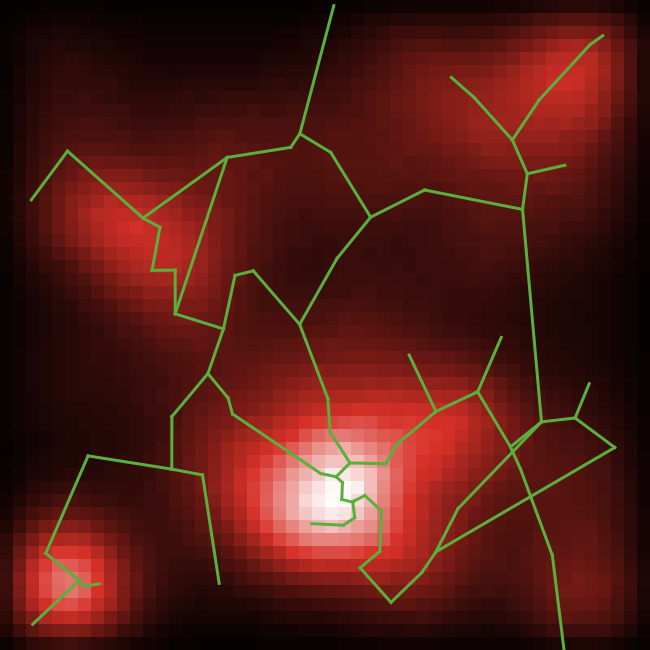
\includegraphics[width=\textwidth]{figures/configs/2_param71913_seed10}\\
$\rho[\bar{d},\bar{c}]\simeq 0.34$
\end{column}%
\hfill%
\begin{column}{.48\textwidth}
\centering
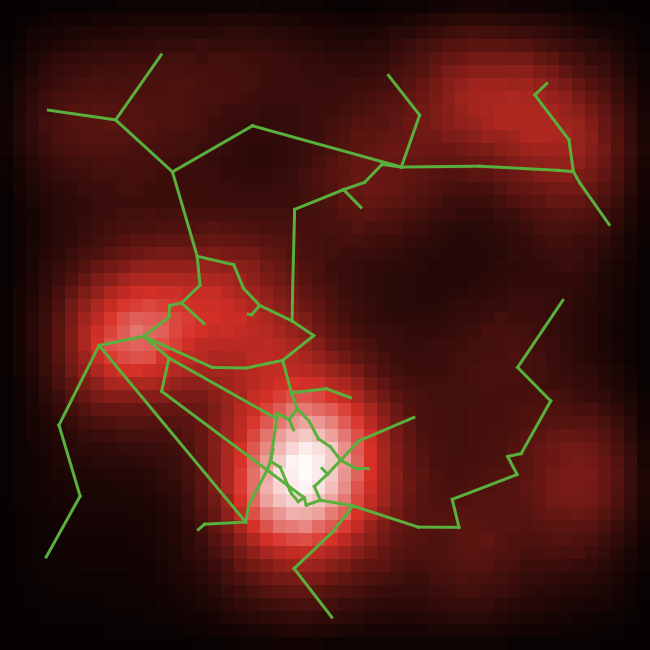
\includegraphics[width=\textwidth]{figures/configs/4_param71945_seed0}\\
$\rho[\bar{d},\bar{c}]\simeq-0.41$
\end{column}%
\end{columns}

$\rightarrow$ \textit{plus forte prégnance de la hiérarchie gravitaire dans (1) $\gamma=3.9,k_h=0.7$ contre $\gamma=1.07,k_h=0.25$ pour (2)}

}






%%%%%%%%%%%%%%%%%
\section{Discussion}
%%%%%%%%%%%%%%%%%

\subsection{Développements}

%%%%%%%%%%%%%%%%%
\sframe{Applications}{
\begin{itemize}
\jitem{\textbf{Cas général : } Sensibilité d'un modèle aux structures de correlations ; contrôle statistique sur correlations.}
\jitem{\textbf{Exemple géographique : } 
\begin{enumerate}
\item Calibration du modèle couplé, données de réseau routier ( ¡ effets de bord !) $\rightarrow $ génération de données synthétiques correspondant à un système urbain donné $\rightarrow$ corrélations intrinsèque à une configuration (à comparer à correlations estimées entre différents états : non-ergodicité des systèmes urbains~\cite{pumain2012urban}).
\item Correlations dynamiques dans un modèle fortement couplé / corrélations spatio-temporelle dans un couplage fort spatial.
\end{enumerate}
}
\jitem{Idées pour vos domaines ?}
\end{itemize}

}

\subsection{Généralisation}

%%%%%%%%%%%%%%%%%
\sframe{Généralisation}{
\textit{Possibilités de généralisation : }
\bigskip
\begin{itemize}
\jitem{Structures de dépendances non-linéaires\\\cite{chicheportiche2013nested}}
\jitem{Contrôle des moments croisés à tout ordre ? Difficile car augmentation rapide du nombre de paramètres nécessaires ; peu d'intérêt ?}
\end{itemize}


}


%%%%%%%%%%%%%%%%%
\sframe{Conclusion}{

% put positioning here

\begin{itemize}
\jitem{Positionnement scientifique : multidisciplinarité (intégration horizontale des systèmes complexes) et modèles computationnels hétérogènes ou multi-échelle (intégration verticale)}
\jitem{Méthode générique appliquée de deux façons : méthode hybride dérivation analytique/simulation ; exploration intensive d'un modèle de simulation.}
\jitem{Retour au ski : type d'approche essentiel pour validation et application de modèles de simulation. Ski ou Snow ?}
\end{itemize}



}



%%%%%%%%%%%%%%%%%
\sframe{Réserve}{

\textbf{Slides de réserve}

}
%%%%%%%%%%%%%%%%%%%%%%%%%%%%




%%%%%%%%%%%%%%%%%
\begin{frame}[allowframebreaks]
\frametitle{Modèle de génération de réseau}
\footnotesize
\begin{enumerate}
\item Un nombre fixé $N_c$ de centres qui seront les premiers noeuds du réseau est distribué selon la distribution de densité, suivant une loi similaire à celle d'agrégation, i.e. la probabilité d'être distribué sur une case est $\frac{(P_i/P)^{\alpha}}{\sum (P_i/P)^{\alpha}}$. La population est ensuite répartie selon les zones de Voronoi des centres, un centre cumulant la population des cases dans son emprise.
\item Les centres sont connectés de façon déterministe par percolation entre plus proches clusters : tant que le réseau n'est pas connexe, les deux composantes connexes les plus proches au sens de la distance minimale entre chacun de leurs sommets sont connectées par le lien réalisant cette distance. On obtient alors un réseau arborescent.
\item Le réseau est alors modulé par ruptures de potentiels afin de se rapprocher de formes réelles. Plus précisément, un potentiel d'interaction gravitaire généralisé entre deux centres $i$ et $j$ est défini par
\[
V_{ij}(d) = \left[ (1 - k_h) + k_h \cdot \left( \frac{P_i P_j}{P^2} \right)^{\gamma} \right]\cdot \exp{\left( -\frac{d}{r_g (1 + d/d_0)} \right)}
\]

où $d$ peut être la distance euclidienne $d_{ij}=d(i,j)$ ou la distance par le réseau $d_N(i,j)$, $k_h \in [0,1]$ un poids permettant de changer le rôle des population dans le potentiel, $\gamma$ régissant la forme de la hiérarchie selon les valeurs des populations, $r_g$ distance caractéristique de décroissance et $d_0$ paramètre de forme.
\item Un nombre $K\cdot N_L$ de nouveaux liens potentiels est pris comme les couples ayant le plus grand potentiel pour la distance euclidienne ($K=5$ est fixé).
\item Parmi les liens potentiels, $N_L$ sont effectivement réalisés, qui sont ceux ayant le plus faible rapport $V_{ij}(d_N)/V_{ij}(d_{ij})$ : à cette étape seul l'écart entre distance euclidienne et distance par le réseau compte, ce rapport ne dépendant plus des populations et étant croissant en $d_N$ à $d_{ij}$ fixé.
\item Le réseau est planarisé par création de noeuds aux intersections éventuelles créées par les nouveaux liens.
\end{enumerate}

\end{frame}

\begin{frame}
\frametitle{Paramètres}
Paramètres de génération de densité $\vec{\alpha}_D = (P_m/N_G , \alpha,\beta , n_d)$ (on s'intéresse pour simplifier au rapport entre population et taux de croissance, i.e. le nombre d'étapes nécessaires pour générer) et des paramètres de génération de réseau $\vec{\alpha}_N=(N_C,k_h,\gamma , r_g , d_0)$. On notera $\vec{\alpha} = (\vec{\alpha}_D,\vec{\alpha}_N)$.
\end{frame}


\begin{frame}
\frametitle{Indicateurs}
\small
On quantifie la forme urbaine et la forme du réseau, dans le but de moduler la corrélation entre ces indicateurs. La forme est définie par un vecteur $\vec{M}=(r,\bar{d},\varepsilon,a)$ donnant auto-corrélation spatiale (indice de Moran), distance moyenne, entropie, hiérarchie (voir~\cite{le2015forme} pour une définition précise de ces indicateurs). Les mesures de la forme du réseau $\vec{G} = (\bar{c},\bar{l},\bar{s},\delta)$ sont, avec le réseau noté $(V,E)$,
\begin{itemize}
\item Centralité moyenne $\bar{c}$, définie comme la moyenne de la \emph{betweeness-centrality} (normalisée dans $[0,1]$) sur l'ensemble des liens.
\item Longueur moyenne des chemins $\bar{l}$ définie par $\frac{1}{d_m}\frac{2}{|V|\cdot (|V|-1)}\sum_{i<j}d_N(i,j)$ avec $d_m$ distance de normalisation prise ici comme la diagonale du monde $d_m=\sqrt{2}N$.
\item Vitesse moyenne~\cite{banos2012towards}, qui correspond à la performance du réseau par rapport au trajet à vol d'oiseau, définie par $\bar{s} = \frac{2}{|V|\cdot (|V|-1)}\sum_{i<j}{\frac{d_{ij}}{d_N(i,j)}}$.
\item Diamètre du réseau $\delta = \max_{ij}d_N(i,j)$
\end{itemize}
\end{frame}





%%%%%%%%%%%%%%%%%%%%%
\begin{frame}[allowframebreaks]
\frametitle{References}
\bibliographystyle{apalike}
\bibliography{/Users/Juste/Documents/ComplexSystems/CityNetwork/Biblio/Bibtex/CityNetwork,biblio}
\end{frame}
%%%%%%%%%%%%%%%%%%%%%%%%%%%%












\end{document}















